\documentclass{article}
\author{Giuliano Abruzzo \\
Basato sugli appunti di Edoardo Puglisi \\ \url{https://github.com/machine1104/masterNotes}}
\title{Web Information Retrieval Notes}
\usepackage{geometry}
\usepackage{float}
\usepackage{graphicx}
\usepackage{amsmath}
\usepackage{hyperref}
\usepackage{algorithm}
\usepackage{color}
\usepackage[table,xcdraw]{xcolor}
\usepackage{amssymb}

\newcolumntype{C}[1]{>{\centering\let\newline\\\arraybackslash\hspace{0pt}}m{#1}}
\newcolumntype{L}[1]{>{\raggedright\let\newline\\\arraybackslash\hspace{0pt}}m{#1}}

\input{insbox}


\begin{document}
\maketitle
\newpage
\tableofcontents
\newpage
\section{Cap 1: Inverted Index \& Boolean Retrieval}
\textbf{Information retrieval} means finding \emph{material} (usually \emph{docs}) of an \textbf{unstructured} (a \emph{data} which doesn't have an easy-for-a-computer \emph{structure}) nature (usually \emph{text}) that satisfies an information need from within large collections. The field of \emph{information retrieval} also covers supporting \emph{users} in \emph{browsing} or \emph{filtering} document collections. Given a set of documents, \textbf{clustering} is the task of coming up with a \emph{good grouping} of the \emph{documents} based on their contents. Given a set of topics, \textbf{classification} is the task of deciding which \emph{class}, if any, each of a set of \emph{documents} belongs to. \emph{Information retrieval} systems can also be distinguished by the \textbf{scale} at which they operate, in \emph{web search}, the system has to provide search over billions of \emph{documents} stored on millions of computers instead at the other extreme there is \emph{personal information retrieval}. \\\\
\textbf{Information retrieval} in the Web is different because:
\begin{itemize}
\item \emph{Infos} can be \textbf{linked};
\item We have huge \emph{sources} with different kinds of files;
\item \emph{Sources} can be not \emph{homogeneous};
\end{itemize}
\emph{Links} can be used for suggestion, from a \emph{page} to another one, every \emph{web page} has a \textbf{rank} that depends on how may \emph{links} point to it, and this \emph{rank} is used by Google for \textbf{relevance criteria}. We can have also a \textbf{quality} difference between \emph{infos} on the same \emph{source}. \emph{Web} in past was different, so now we can distinguish:
\begin{itemize}
\item \textbf{Web 1.0}:
\begin{itemize}
\item In 90s, \emph{infos} on the \emph{web} were almost always generated from a \emph{source} instead \emph{users} were quite passive, in fact web was used for reading, owning, consuming, so very few interactions of the \emph{user}. The \emph{web} was structured in a \emph{hierarchical} way, called \textbf{Taxonomy}.
\end{itemize}
\item \textbf{Web 2.0}:
\begin{itemize}
\item Now, a lot of\emph{ web content} is \textbf{user-generated} and there are a lot of interactions between \emph{users} and \emph{information} that we can retrieve. The structure is not anymore \emph{hierarchical}, we have \emph{tags} and every \emph{tag} is a \emph{category}, this structure is called \textbf{Folksonomy}.
\end{itemize}
\end{itemize}
If we consider the \emph{web} as a \textbf{graph}, where the \emph{nodes} are the \emph{pages} and \emph{edges} are the \emph{hyperlinks} between them:
\begin{itemize}
\item \textbf{Crawling the web} means that by visiting this \emph{graph} we will collect a \textbf{web corpus} (\emph{multiple documents}), starting from a \emph{page} and through this \emph{links} we iterate on another \emph{pages}. Often we don't want to \emph{crawl} some \emph{pages}, cause we don't need them, or we want to add some kind of \emph{restrictions}, and we need to be sure to visit all \emph{relevant pages} in order to avoid \emph{information missing}, so this problem requires an huge amount of \emph{computing power} and \emph{competitiveness};
\item We also need \textbf{Indexing the web}, so we need to give a \emph{structure} to the \emph{web corpus} that we crawled;
\item Last, we need some \textbf{Search Algorithms}, in order to solve \emph{user's information need} using \emph{queries}, they need to be based on \textbf{relevance} (results are coherent with the query) and \textbf{authority} (pages must give user real information);
\end{itemize}  
The \textbf{Meta-Search} is when we research using combined results from multiple \emph{search engines}. A \textbf{collection} is a set of \emph{documents}, not always \emph{static}, and the \textbf{goal} is to collect \emph{documents} that are relevant to\emph{ user's information} need. The \textbf{classic Search Model} is:\\
\begin{tabular}{C{7cm}  L{8cm}}
        \includegraphics[scale=0.5]{cattura1.png} & For example, the \textbf{user task} is: `\emph{how to get rid of a mice in a politically correct way}`, so the \textbf{info need} is `\emph{remove mouse without killing it}`, the \textbf{query} will be `\emph{how trap mouse alive}`\\
\end{tabular}\\\\
Between \textbf{user task} and \textbf{query} there could be some \emph{misconception} or \emph{misformulation} by the \emph{search engine}. In order to measure a \textbf{search engine performance}, we have to compare the \emph{ground truth} (what we expect from a search), with the \emph{result} we actually obtain, and this is done through \textbf{Precision} and \textbf{Recall}:
\begin{itemize}
\item \textbf{Precision}: $\frac{relevant\;docs}{returned\;docs}$
\item \textbf{Recall}: how many documents over the relevant ones are shown;
\end{itemize}
\begin{figure}[H]
  \centering
  \includegraphics[scale=0.8]{cattura2.png}
\end{figure}
Usually we have a \textbf{trade-off} between them, so we need to obtain either a good \emph{precision} or \emph{recall} depending on the problem's type.\clearpage
\hfill \\ The first type of \emph{query} we are going to see is the \textbf{Boolean IR query}, a \emph{query} in which we research \emph{keywords} in \emph{documents}. For example we want to know which plays of Shakespeare contains `\emph{brutus}` \textbf{and} `\emph{caesar}` \textbf{and} \textbf{not} `\emph{calpurnia}`. A way could be \textbf{grepping} (search a \emph{string} in a \emph{document}) all the \emph{plays}, but this is \textbf{strongly inefficient} for large \emph{docs} and it's not flexible for other \emph{matching operations}. Another option is using a \textbf{binary term-document incidence matrix}, where the \emph{words} are the \emph{rows}, and the \emph{plays} are the \emph{column}, and we will have a 1 in the cell if that \emph{word} appear in that \emph{play}:\\\\
\begin{tabular}{C{8cm}  L{6.5cm}}
        \includegraphics[scale=0.7]{cattura3.png} & 
        In order to \emph{answer} the \textbf{query} we will take the vectors of \emph{brutus}, \emph{caesar} and \emph{calpurnia} and we do a \emph{bitwise and}: 101000 AND 110111 AND (NOT 010000) = 100100, so the answer will be \emph{Antony and Cleopatra} and \emph{Hamlet}. 
\end{tabular}\\\\
But if we have \textbf{big collection}, we will have a \emph{matrix} too big to fit in a \emph{computer memory}, and also it will be full of \emph{zeroes}, with few \emph{non-zero entries}. A much better representation is to record only the\emph{ 1's occurrences}, by using an \textbf{Inverted Index}:\\\\
\begin{tabular}{C{8cm}  L{6.5cm}}
        \includegraphics[scale=0.65]{cattura4.png} & 
       This means that for each \emph{term} we will have a \emph{linked list }that records which \emph{documents} the \emph{term} occurs in. Every \emph{document} must have a \textbf{docID} that identify it and these are \emph{sorted}, so we avoid to use \emph{fixed length array}.
\end{tabular}\\\\
In order to build an \textbf{inverted index} we need to:\\
\begin{tabular}{C{7cm}  L{6.5cm}}
        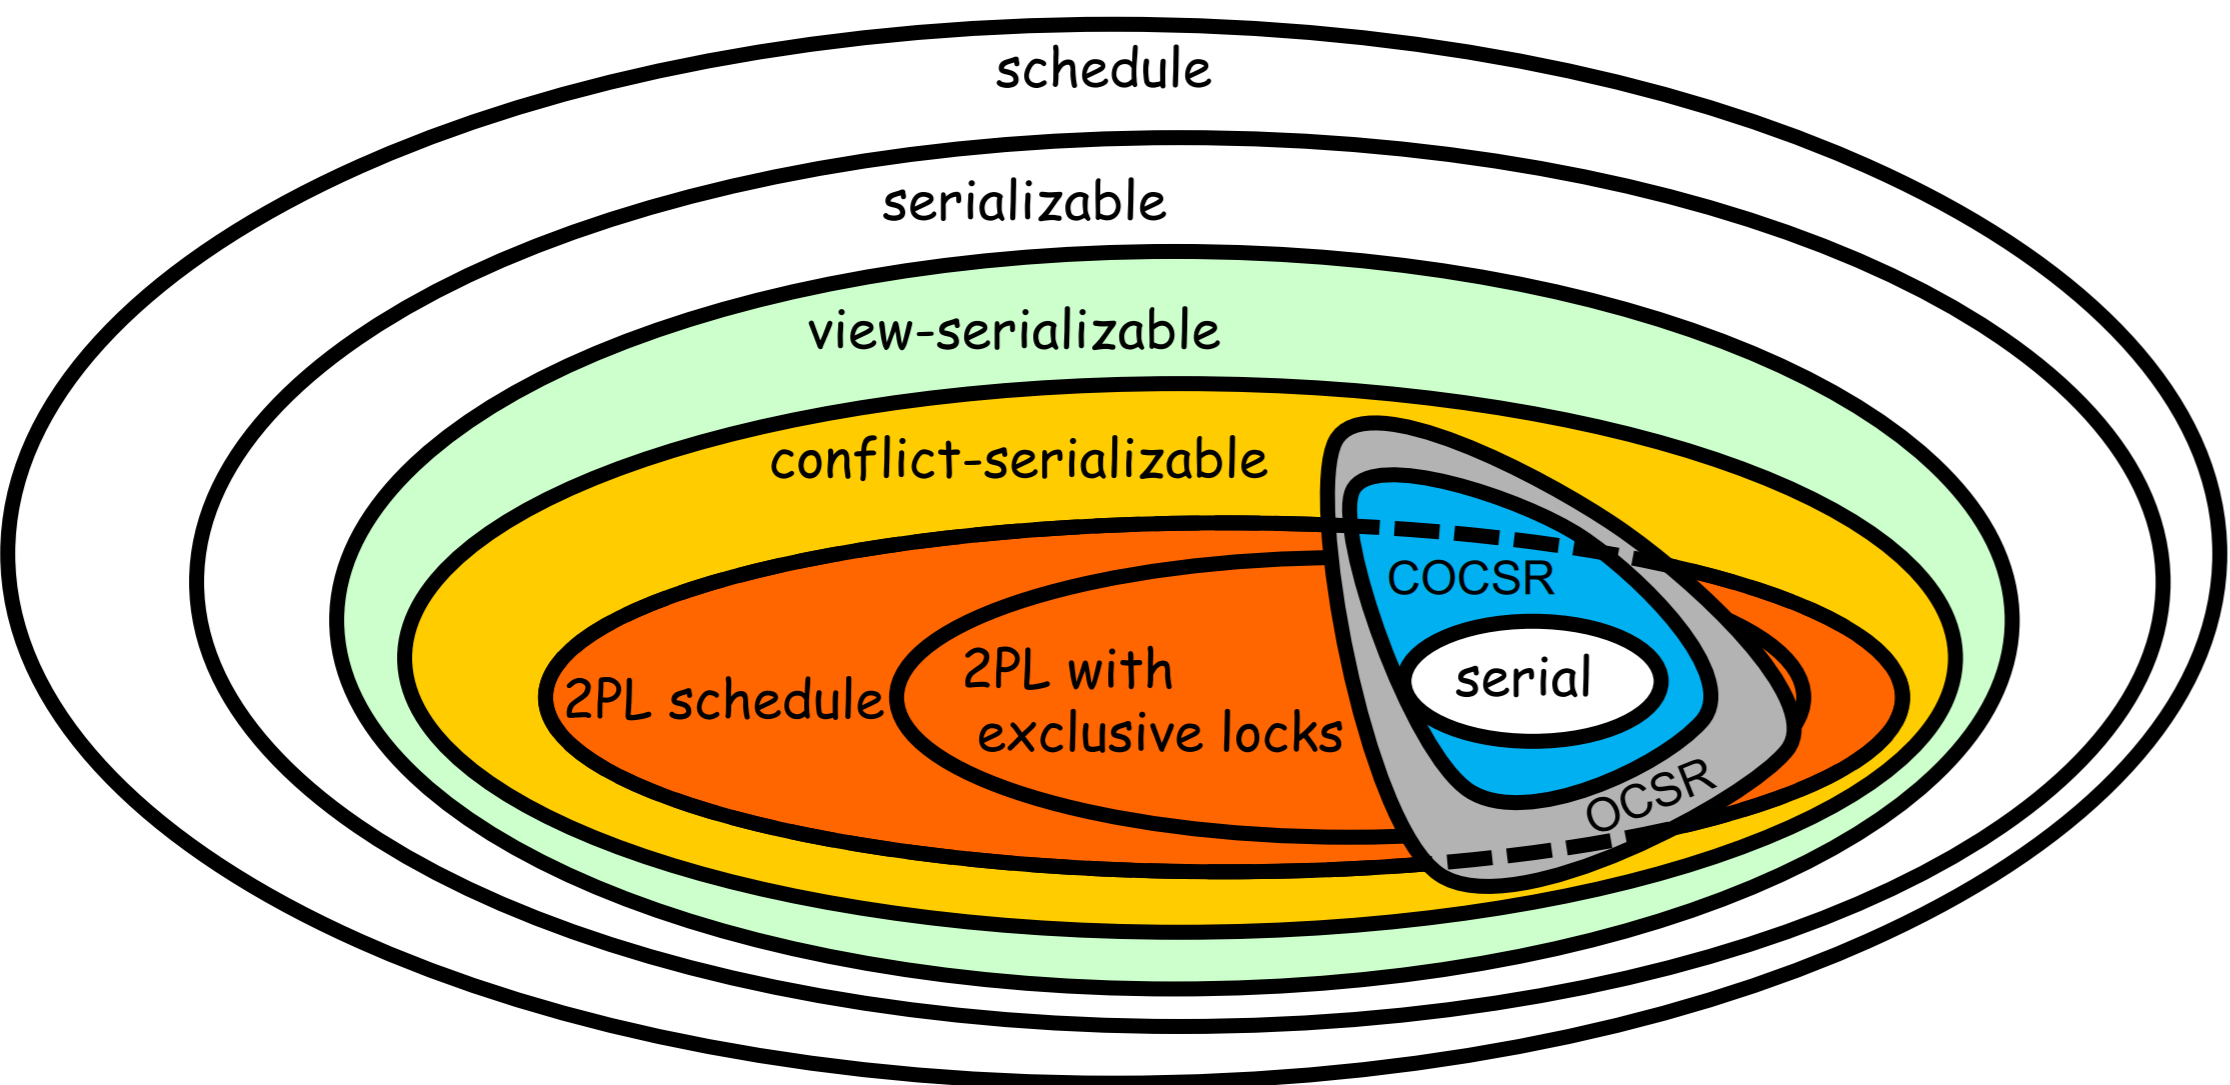
\includegraphics[scale=0.6]{cattura5.png} & 
	\begin{itemize}
	\item Collect the \emph{documents} to be \emph{indexed};
	\item \emph{Tokenize} the \emph{text}, turning each \emph{document} into a list of \emph{tokens};
	\item Do \emph{linguistic preprocessing}, producing a list of \emph{normalized tokens}, which are the \emph{indexing terms};
	\item Index the \emph{documents} that each term occurs in by creating an \emph{inverted index}, consisting of a \emph{dictionary} and  \emph{postings}.
	\end{itemize}
\end{tabular}
\clearpage
\hfill \break
In \emph{linguistic modules} we \textbf{stem} the text and also remove \emph{stopwords}, not only \emph{lowercase}. The core \textbf{indexing step} is \emph{ordering} both \emph{words} and \emph{docID}, and often also the \emph{frequency} of every \emph{word} is added. So the \emph{cost} for a \emph{query} $word1\; AND\; word2 $is $O(X+Y)$ where $X$ and $Y$ are the \emph{postings length} of the two \emph{words}. The \emph{intersect} of the two \emph{posting lists} is the crucial operation, and it's also called \textbf{merging}. The \textbf{query optimization} is the process of selecting how to organize the work of answering a \emph{query}:
\begin{itemize}
\item \textbf{(... AND ...) AND (... AND ...):} we will start from \emph{intersect} the two smallest \emph{posting lists}, so the next \emph{intersection} will be more efficient;
\item \textbf{(... OR ...) AND (... OR ...):} we use the \emph{frequency} to estimate which \emph{OR} we will use, usually the one which \emph{term's frequency sum} is lower;
\end{itemize}
Sometimes we want a \emph{query} to match a \emph{phrase}, for example we want to answer queries with `\emph{stanford university}`, we call these  \textbf{Phrase Queries}. These \emph{words} have to appear in these \emph{precise order}, so a \emph{posting list} is not good anymore, we could index every consecutive pair of \emph{terms} in the \emph{text} as a \emph{phrase}, also called \textbf{Biword Indexes}, for example `\emph{Friends, Romans, Countryman}` generate two biwords `\emph{friends romans}` and `\emph{romans countryman}`, where each of these is a \emph{dictionary term}, but we will have too many \emph{dictionaries} and \emph{false positive}. So we need to use a \textbf{Positional Index}, in which we consider the \textbf{position} of the \emph{term} in the \emph{docs}:\\\\
\begin{tabular}{C{7cm}  L{6.5cm}}
        \includegraphics[scale=1]{cattura6.png} & 
	Where at the left we have \emph{docID}, at the right the \emph{positions} of the \emph{word}. Using position we can even do \textbf{proximity search} and we can also combine \emph{Biword} and \emph{Positional}.
\end{tabular}\\\\
\section{Cap 2: Document Ingestion}
\subsection{Tokenization}
We said that in order to construct an \emph{inverted index}, we need to \textbf{tokenize} the \emph{text}. \textbf{Tokenization} is the process of chopping \emph{character streams} into \emph{tokens}, a \textbf{token} is a sequence of chars grouped together as a \emph{semantic unit} for \emph{processing}. \emph{Tokenization} depends on how we want to process the \emph{index} (by \emph{words}, by \emph{biwords}, ...), the most simple strategy is to split on \emph{whitespaces}, but there could be the need of grouping special sets of \emph{characters}. The problem of \emph{tokenization} is finding the correct \emph{token} to use, for `\emph{Finland's}` which is the best \emph{tokenization}? `\emph{Finland AND s}`, `\emph{Finlands}` or `\emph{Finland's}`, these issues are \textbf{language-specific}, so we require to know the \emph{language} of the document, we can have also problems with \emph{dates} and \emph{numbers}. 
\subsection{Stopwords}
\textbf{Stopwords} are \emph{words} that are extremely common and their \emph{semantic content} is almost useless, they are generated by \emph{collection frequency} (number of times each \emph{term} appears in \emph{documents}). Using a \emph{stop list }significantly reduces the number of \emph{postings} that a \emph{system} has to store, and a lot of the time not indexing \emph{stop words} does little harm: keyword searches with terms like \emph{the} and \emph{by} don’t seem very useful. However, this is not true every time, for example, the meaning of \emph{flights to London} is likely to be lost if the word \emph{to} is stopped out. For most modern \emph{IR systems}, the additional cost of including \emph{stop words} is not that big, neither in terms of \emph{index size} nor in terms of \emph{query processing time}.
\subsection{Normalization}
\textbf{Normalization} is the process of canonize \emph{tokens} so that matches occur despite superficial differences in the character sequences of the \emph{tokens}. The most standard way to \emph{normalize} is to implicitly create \textbf{equivalence classes}, for example we delete dots (\emph{U.S.A} $\rightarrow$ \emph{USA}) or hyphens (\emph{anti-discriminatory} $\rightarrow$ \emph{antidiscriminatory}). It can also be applied on accents or variants and there could misunderstanding too, but even on \emph{synonyms}. During \emph{normalization} all \emph{token} characters are reduced to \emph{lower case}.
\subsection{Stemming and Lemmatization}
For grammatical reasons, \emph{documents} are going to use different forms of a \emph{word}, such as \emph{organize}, \emph{organizes}, and \emph{organizing}. The goal of both \textbf{stemming} and \textbf{lemmatization} is to reduce \emph{inflectional forms}, for instance: \emph{am}, \emph{are}, \emph{is} $\rightarrow$ \emph{be}, or \emph{car}, \emph{cars}, \emph{car's}, \emph{cars' }$\rightarrow$ \emph{car}. \textbf{Stemming} usually refers to a heuristic process that \emph{chops off} the ends of \emph{words} in the hope of achieving this goal correctly most of the time, includes the removal of \emph{derivational affixes}. \textbf{Lemmatization} usually refers to doing things properly with the use of a \emph{vocabulary} and \emph{morphological analysis} of \emph{words}, normally aiming to remove inflectional endings only and to return the base or \emph{dictionary} form of a \emph{word}, which is known as the \textbf{lemma}. The most common algorithm for \emph{stemming} English is \textbf{Porter's Algorithm}, which consists of 5 phases of \emph{word reductions}, applied sequentially, some typical rules are: substitution like $SSES \rightarrow SS$ or $IES \rightarrow I$, weight of word sensitive rules, ($m > 1$) Ement: $replacement \rightarrow replac$ or $cement \rightarrow cement$. 
\subsection{Faster Postings List}
In the basic \textbf{postings list intersection}, if the list lengths are \emph{m }and \emph{n}, the \emph{intersection} takes $O(m+n)$ operations. One way to do better than this is to use a \textbf{skip list} by augmenting \emph{postings lists} with \textbf{skip pointers} (at indexing time), which allow us to avoid \emph{processing parts} of the \emph{postings list} that will not figure in the \emph{search results}. We have a \emph{trade-off}, more \emph{skips} means shorter\emph{ skip spans} (space of a skip), but also means lot of \emph{comparisons} and lots of space storing \emph{skip pointers}. Building effective \emph{skip pointers} is easy if an \emph{index} is relatively static, it is harder if a \emph{postings list} keeps changing because of updates.
\begin{figure}[H]
  \centering
  \includegraphics[scale=0.6]{cattura7.png}
\end{figure}
\clearpage
\section{Cap 3: Dictionaries and Tolerant Retrieval}
\subsection{Dictionaries}
\textbf{Data Structure} for \emph{posting lists} are usually \emph{dictionaries}, but we need to store in memory efficiently, and also we need to quickly look up elements at \emph{query time}. There are two main choices: \textbf{Hash Tables} and \textbf{Trees}:
\begin{itemize}
\item \textbf{Hash Tables}:
\begin{itemize}
\item Each \emph{vocabulary term} (the \textbf{key}) is \textbf{hashed} into an \emph{integer} over a large enough \emph{space} (in order to avoid \emph{hash collisions}), at \emph{query time} we \emph{hash} each \emph{query} term separately and following a \emph{pointer} to the corresponding \emph{postings}. So the \emph{lookup} is really fast $O(1)$, the problem is that it's not easy to find \emph{similarity} (minor variants of a \emph{query term}), and there is no \emph{prefix search}. If the size of the \emph{vocabulary} keeps growing we may need to \emph{rehash} everything to avoid \emph{collisions}. 
\end{itemize}
\item \textbf{Trees}:
\begin{itemize}
\item The best-known \emph{search tree} is the \textbf{binary tree}: the search for a \emph{term} begins at the \emph{root} of the \emph{tree}, each \emph{internal node} (including the \emph{root}) represents a \emph{binary test}. A \textbf{lookup} costs $O(log\;N)$ if the \emph{tree} is \textbf{balanced} (number of \emph{terms} under the two \emph{sub-trees} of any \emph{node} is equal or differ by one), else is $O(N)$. It solves the \emph{prefix search} problem, but we can have problems of\emph{ re-balancing}, in fact when we insert new \emph{terms} or we delete old ones the \emph{tree} needs to be re-balanced. One approach to avoid it is to allow the number of \emph{sub-trees} under an \emph{internal node} to vary in a fixed interval, these are called \textbf{B-Trees}, in which every \emph{internal node} has a number of children in the interval $\left [a,b\right]$. Unlike \emph{hashing}, \textbf{search trees} demand that the characters used in the document collection have a \textbf{prescribed ordering}.
 \begin{figure}[H]
  \centering
  \includegraphics[scale=0.6]{cattura8.png}
\end{figure}
\end{itemize}
\end{itemize}
\subsection{Wild-Card Queries}
\textbf{Wildcard Queries} are used in any of the following situations:
\begin{itemize}
\item The user is uncertain of the spelling of a \emph{query term}, like \emph{Sydeny} vs \emph{Sidney}, so the wildcard query is \emph{S*dney};
\item The user is aware of multiple variants of spelling a term, and seeks documents containing any of the variants, like \emph{color} vs \emph{colour};
\item The user seeks documents containing variants of a term that would be caught by \emph{stemming}, but is unsure whether the search engine performs stemming like \emph{judicial} vs. \emph{judiciary}, the wildcard query \emph{judicia*}; 
\item The user is uncertain of the correct rendition of a foreign word or phrase, like \emph{Universit* Stuttgart};
\end{itemize}
A \emph{query} such as \emph{mon*} is \textbf{trailing wildcard query}, because the \emph{* symbol} occurs only once, at the end of the search \emph{string}. This query is easy to find in a B-tree, but the query \emph{*mon} is very harder, called \textbf{leading wildcard queries}, we can use a reverse \emph{B-Tree} in which each \emph{root-to-leaf} path corresponds to a term written backwards, for example \emph{lemon} will be represented by the path \emph{root-n-o-m-e-l}. Using a regular\emph{ B-Tree} together with a \emph{reverse B-Tree} we can handle a general case \emph{se*mon} where the regular B-tree is used to find the prefix \emph{se}, and the reverse B-tree is used to find the suffix \emph{mon}, and then we will \textbf{intersect} the two \emph{sets} obtained, but this solution is pretty expensive. \\\\
A more efficient way is using \textbf{Permutation Index}, a form of \emph{inverted index}, we will use a special symbol $\$$ used to mark the end of a term.\\
\begin{tabular}{C{7cm}  L{6.5cm}}
        \includegraphics[scale=1]{cattura9.png} & 
	If we have to search \emph{hel*o}, the key is to rotate in such a way the \emph{* symbol} is at the end of the string, we set $X = hel$ and $Y=o$, we search for $Y\$X*$ so \emph{o$\$$hel*}. \emph{we search in the regular b-tree, all the words that start with hel and ends with o (? probably?).}
\end{tabular}\\\\
If we have a query like \emph{fi*mo*er} first we ignore the $mo$, and we search for \emph{fi*er} that permuted is \emph{er$\$$fi*}, then we will filter the words that doesn't contain \emph{mo}. The problem with permutation index is that its dictionary becomes quite large.\\\\
In order to solve this problem, we can use the \textbf{Bigram Index} (or\textbf{ K-gram Index} where \emph{k-gram} is a sequence of \emph{k} characters) for a single word, for example in `\emph{April is the cruelest month}`, we get the bigrams: `\emph{$\$$a,ap,pr,ri,il,l$\$$,$\$$i,is,s$\$$,$\$$t,th,he,e$\$$,$\$$c,cr,ru,ue,el,le,es,st,t$\$$, $\$$m,mo,on,nt,h$\$$}`. We maintain a \emph{second inverted index} from \emph{bigrams} to \emph{dictionary terms} that match each \emph{bigram}. For example \emph{$\$$m} will point to \emph{mace}, \emph{madden}, \emph{mo} will point to \emph{among}, \emph{amortize}, $on$ to $along, among$. The query \emph{mon*} can now be run as \emph{$\$$m} AND \emph{mo} AND \emph{on}, but these can return also the word \emph{moon}, so we need another filter at the end. This method is \emph{fast} and \emph{space efficient} (compared to \emph{permutation}). The processing of a \emph{wildcard query} can be quite expensive because of the added \emph{lookup} in the \emph{special index}, \emph{filtering} and finally the \emph{standard inverted index}. A \textbf{search engine} may support such rich functionality, but most commonly, the capability is hidden behind an interface that most users never use.
\subsubsection{Spelling Correction}
There are two methods to solve the problem of \textbf{correcting spelling} errors in \emph{queries}: the first based on \textbf{edit distance} and the second based on\textbf{ k-gram overlap}. There are two basic principles underlying most spelling correction algorithms:
\begin{itemize}
\item Correct spellings for a \emph{misspelled query}, so we choose the \textbf{nearest one}; 
\item When two correctly spelled \emph{queries} are tied, select the one that is \textbf{more common};
\end{itemize}
We will focus on two types of \emph{spelling correction}: \textbf{isolated-term correction} and \textbf{context-sensitive correction}:
\begin{itemize}
\item \textbf{Isolated-Term correction}: 
\begin{itemize}
\item  In \textbf{isolated-term correction}, we attempt to correct a single \emph{query term} at a time, but such \emph{isolated-term correction} would fail to detect, for instance, that the query \emph{flew form Heathrow} contains a misspelling of the term \emph{from}, because each term in the \emph{query} is correctly spelled in isolation.
\item \textbf{Edit Distance}:
\begin{itemize}
\item Given two strings $s_1$ and $s_2$, the \textbf{edit distance} between them is the minimum number of \emph{edit operation} to convert one string to the other. \emph{Edit distance} is also called \textbf{Levenshtein distance}, for example the edit distance of \emph{cat} and \emph{dog} is 3. There is also the \textbf{weighted edit distance} in which we have a \emph{weight} based on the \emph{character} involved (char $m$ mis-typed as $n$ more than $z$, so replacing $m$ with $n$ is a smaller edit then $z$), but these requires a \emph{weight matrix} as input. In order to compute the\emph{ weighted edit distance} we need $O(|s_1| \times |s_2|)$ where $|s_1|$ denotes the length of the string. In order to correct the \emph{spelling}, given a \emph{query}, first we enumerate all \emph{char sequences} within a preset \emph{weighted edit distance}, then we intersect this set with list of \emph{correct words}, then we show these \emph{words} to the user as a suggestion. 
\end{itemize}
\item \textbf{N-Gram Overlap}:
\begin{itemize}
\item We can use the \textbf{n-gram index} to retrieve \emph{vocabulary terms} that have many\emph{ n-grams} in common with the \emph{query}, and the \emph{retrieval process} is essentially that of a single scan through the \emph{postings} for the\emph{ n-grams} in the \emph{query string}. For example if the text is \emph{november} (trigrams are \emph{nov, ove, vem, emb, mbe, ber}) and the query is \emph{december} (trigrams are \emph{dec, ece, cem, emb, mbe, ber}) so we have 3 \emph{trigrams} that overlap. The measure of \emph{overlapping} is given by the \textbf{Jaccard Coefficent} by two sets $X$ and $Y$ and it is: $|X \cap Y| \setminus |X \cup Y|$, this will be a value between 0 and 1, so we will choose the \emph{terms} over a certain \emph{threshold}. 
\end{itemize}
\end{itemize}
\item \textbf{Context-Sensitive Correction}:
\begin{itemize}
\item \emph{Isolated-term correction} would fail to correct typographical errors where all \emph{query terms} are correctly spelled, for example `\emph{I flew form Milan}`, `\emph{form}` is an error (\emph{from}). The simplest way to correct these errors is to enumerate \emph{corrections} of each of the \emph{query terms} even though each \emph{query term} is correctly spelled, then try substitutions of each \emph{correction} in the phrase. For each such \emph{substitute phrase}, the \emph{search engine} runs the \emph{query} and determines the number of \emph{matching results}. This enumeration can be expensive, several \emph{heuristics} are used to reduce the \emph{search space}. We wanna rank alternatives probabilistically: $argmax_{corr}\; P(corr|query)$, that with bayes rules is: $argmax_{corr}\;P(query|corr)*P(corr)$, where \emph{query} is the noisy channel, and \emph{corr} the language model.
\end{itemize}
\end{itemize}
\subsubsection{Phonetic Correction}
Misspellings that arise because the user types a \emph{query} that sounds like the \emph{term target}. The main idea here is to generate, for each term, a \textbf{phonetic hash} so that \emph{similar-sounding terms hash} to the same value. Algorithms for such \emph{phonetic hashing} are commonly collectively known as \textbf{Soundex algorithms}, common steps are:
\begin{itemize}
\item We turn every \emph{term} to be indexed into a \emph{4-character reduced form}, we build an \textbf{inverted index} from these reduced forms to the original \emph{terms} called \emph{soundex index}.;
\item We do the same with the \emph{query terms};
\item When the \emph{query} calls for a \emph{soundex match}, search this \emph{soundex index};
\end{itemize}
\section{Cap 4: Index Construction Algorithm}
In order to answer a \emph{query}, we need to build an \emph{inverted index} for a set of terms, this construction process is called \textbf{Index Construction} or \textbf{Indexing}, that takes advantage of \emph{secondary storage}. It's important to note that:\emph{ main memory} $>>>$ \emph{secondary storage}, it's way faster. There are some consideration:
\begin{itemize}
\item To optimize \textbf{transfer time} we have a big \emph{chunk} of data and not several small \emph{chunks};
\item \textbf{Disk I/O} is \emph{block-based} (of fixed lights);
\item \textbf{Fault tolerance} is handled with \emph{replication} (several instead of a single fault-tolerant machine);
\item The \textbf{main memory} is the better;
\end{itemize}
We need larger average \emph{word token} \emph{size} to handle \emph{words}, especially if we strip out \emph{stepwords}. The goal is construct the \emph{inverted index}, but we can't do the whole sorting in \emph{main memory}, we need intermediate steps. 
\subsection{BSBI Algorithm}
\textbf{BSBI Algorithm} or \textbf{Blocked Sort-Based Indexing Algorithm}, is an \textbf{external sorting algorithm} which try to minimize the number of \emph{random disk seeks }during \emph{sorting}, for example to sort \emph{100M postings} (made of pairs \emph{term-docID}) we define \emph{10 blocks} of \emph{10M postings} each, in such a way that each \emph{block} can fit in the \emph{memory} and:
\begin{itemize}
\item For each \emph{block}:
\begin{itemize}
\item Accumulate \emph{postings};
\item Sort in \emph{memory};
\item Write to \emph{disk};
\end{itemize}
\item Then merge all the \emph{blocks sorted} in order to obtain the \emph{final index};
\end{itemize}
\clearpage
 \begin{figure}[H]
  \centering
  \includegraphics[scale=1]{cattura10.png}
\end{figure}
The \emph{algorithm} parses \emph{documents} into \emph{termID–docID} (\emph{termID is a unique mapped in a dictionary from the term}) pairs and accumulates the pairs in \emph{memory} until a \emph{block} of a fixed size is full, the \emph{block} is then inverted and written to \emph{disk}. \textbf{Inversion} involves two steps, first we sort the \emph{termID–docID pairs}, next, we collect all \emph{termID–docID} pairs with the same \emph{termID} into a \emph{postings list}, where a \emph{posting} is simply a \emph{docID}, and the result is then written to \emph{disk}. In the final step, the algorithm simultaneously merges the \emph{blocks} into one large \emph{merged index}. It's time complexity is $O(T\; log\;T)$, cause the step with the \emph{highest time complexity} is \emph{sorting}, and $T$ is an \emph{upper-bound} for the number of \emph{items} we must sort. The actual \emph{indexing time} is usually dominated by the time it takes to parse the document (\emph{parse block function}), and the final merge (\emph{merge blocks function}). The key decision is the \textbf{block size} that need to be \emph{optimized}. 

\subsection{SPIMI Algorithm}
\emph{Blocked sort-based indexing} has excellent \emph{scaling properties}, but it needs a \emph{data structure} for mapping \emph{terms} to \emph{termIDs}. For very large collections, this \emph{data structure} does not fit into \emph{memory}. An alternative is \textbf{Single-Pass In-Memory Indexing or SPIMI}, which uses separate \emph{dictionaries} for each \emph{block} (so we don't need to maintain \emph{term-termID} mapping across \emph{blocks} like in \emph{BSBI}), and the other idea is \textbf{don't sort}, so we accumulate \emph{postings} in \emph{postings lists} as they occur, so we can generate a complete \emph{inverted index} for each \emph{block} that we will merge into one \emph{big index}. Each \emph{postings list} is dynamic so it's immediately available to collect \emph{postings}, and this has two advantages, it's \emph{faster} (no sorting) and saves \emph{memory} cause we keep track of the term a \emph{posting lists} belongs to, so the \emph{termID} of postings doesn't need to be stored. \emph{SPIMI} has also an important component, the \textbf{compression}, in fact both \emph{postings} and the \emph{dictionary terms} can be store compactly on \emph{disk}. The \emph{time complexity} is $O(T)$ since no sorting is required and all operations are linear in the size of the collection. \emph{SPIMI\_INVERT} is called repeatedly on the \emph{token stream} until the entire \emph{collection} has been processed. \emph{Tokens} are processed one by one during each successive call of \emph{SPIMI\_INVERT}. When a \emph{term} occurs for the first time, it is added to the \emph{dictionary}, and a new \emph{postings list} is created, at the end it returns this \emph{postings list} for subsequent occurrences of the term. (\emph{NOT SURE} \emph{we don't sort postings cause they are already sorted by the docsID that is incremental when received})
 \begin{figure}[H]
  \centering
  \includegraphics[scale=1]{cattura11.png}
\end{figure}
\subsection{Distributed Indexing}
\emph{Collections} are often so large that we cannot perform \textbf{index construction} efficiently on a \emph{single machine}, in this case we will use \textbf{distributed indexing algorithms} for \emph{index construction}. The result of the construction process is a \emph{distributed index} that is partitioned across several machines. We have a \textbf{Master Machine} which is a \emph{fault-tolerant machine}, and \textbf{Idle Machines}, that are part of a \emph{pool} and they have \emph{indexing tasks} in parallel assigned by the \emph{master}. \\\\ The distributed index construction method is an application of \textbf{MapReduce} a general architecture for \emph{distributed computing}.  A robust \emph{distributed indexing} needs the work to be divided in re-assignable chunks, a \textbf{master node} directs the process of assigning and reassigning \emph{tasks} to individual \textbf{worker nodes} (\emph{idle machine}). \\\\First, the input data, are split into \emph{n splits} where the size of the \emph{split} is chosen to ensure that the work can be distributed evenly and efficiently, these \emph{splits} are not preassigned to \emph{machines}, but are instead assigned by the \emph{master node}: as a \emph{machine} finishes processing one \emph{split}, it is assigned the next one, if a machine dies, the \emph{split} it is working on is simply reassigned to another machine. In general, \emph{MapReduce} breaks a large computing problem into smaller parts by \emph{recasting} it in terms of manipulation of\emph{ key-value pairs}, in the form of $\left \langle termID, docID \right \rangle$. \\\\The \textbf{map phase} consists of \emph{mapping splits} of the input data to \emph{key-value pairs}, the machines that execute the map phase are called \textbf{parser}. Each \emph{parser} writes its output to local intermediate files, the \emph{segment files}. For the \textbf{reduce phase}, we want all values for a \emph{given key} to be stored close together, this is achieved by \emph{partitioning} the \emph{keys} into $j$ \emph{term partitions} (\emph{range of letters like a-f}) and having the \emph{parsers} write \emph{key-value pairs} for each term \emph{partition} into a separate \emph{segment file}. Collecting all values for a \emph{given key} into one list is the task of the \textbf{inverters}, the \emph{master} assigns each \emph{term partition} to a different \emph{inverter}. Finally, the list of \emph{values} is sorted for each \emph{key} and written to the final \emph{sorted postings list}. \emph{Parsers} and \emph{inverters} are not separate sets of machines, the \emph{master} identifies \emph{idle machines} and assigns \emph{tasks} to them, the same machine can be a \emph{parser} in the \emph{map phase} and an \emph{inverter} in the \emph{reduce phase}.
\begin{figure}[H]
  \centering
  \includegraphics[scale=1]{cattura12.png}
\end{figure}
\subsection{Dynamic Indexing}
Most collections are \emph{modified frequently} with \emph{documents} being \emph{added, deleted}, and \emph{updated}, new \emph{terms} need to be added to the \emph{dictionary}, and \emph{postings lists} need to be updated. The simplest way to achieve this is to \emph{periodically reconstruct} the \textbf{index} from scratch, this is a good solution if the number of changes over time is small and if enough resources are available to construct a new \emph{index} while the old one is still available for \emph{querying}.\\\\ If there is a requirement that new \emph{documents} be included quickly, the simplest approach is to use \emph{two indexes}, a large \textbf{main index} on \emph{disk}, and a small \textbf{auxiliary index} that store new documents in \emph{memory}. \emph{Searches} are run across both \emph{indexes}, \emph{deletions} are stored in an \textbf{invalidation bit vector}, then we filter out \emph{deleted documents} before returning the \emph{search} result. When the \emph{auxiliary index} becomes too large, we merge it with the \emph{main index}. Unfortunately, this scheme is infeasible because most \emph{file systems} cannot efficiently handle very large numbers of files and merges are computationally expensive. The simplest alternative is to store the \emph{index} as one large file as a concatenation of all \emph{postings list}, but this would generate a lot of files. \\\\
An alternative is the \textbf{Logarithmic Merge}, that reduces the cost of \emph{merging indexes} over time. We maintain \emph{several indexes}, \textbf{each twice larger than the previous one}, and the smallest $Z_0$ is maintained in memory , and the others ($I_0, I_1, ...$) are on disk, when $Z_0$ becomes too large, we will write it to disk as $I_0$, or we merge it with $I_0$ if it already exist and write the merger to $I_1$ and so on. It use a \emph{binary number} to save which index is full for example $1011$ (positions 3 2 1 0), means that $I_2$ has space, instead the others are full. For example if we have $a$ as size of a \emph{memory index}, then on the \emph{disk} we will have \emph{indexes} of size $2a$, $4a$ and so on, so \emph{logarithmic scale}. The \textbf{time complexity} of \emph{index construction} in the worst case is $O(T\; log T)$, because $log\; T$ is the number of indexes with $T$ number of postings, so for a query we need to merge $O(log\; T)$ indexes and the worst case is $O(T\; log\; T)$ because each of $T$ posting is merged $O(log\; T)$ times. This is more efficient than the $O(n^2)$ of the previous alternative. (\emph{supponiamo che una parola ha $T$ postings nella sua posting list, se devo fare il merge su tutte le $I_i$ allora avrò $T\: log T$ dato che i vari $I_i$ sono ognuno il doppio del precedente})
\begin{figure}[H]
  \centering
  \includegraphics[scale=1]{cattura13.png}
\end{figure}
Because of this \emph{complexity} of \emph{dynamic indexing}, some large search engines adopt a \textbf{reconstruction from-scratch strategy}. They do not construct \emph{indexes dynamically}, instead, a new \emph{index} is built from scratch periodically. \emph{Query processing} is then switched from the \emph{new index} and the \emph{old index} is deleted.
\newpage
\section{Index Compression Algorithms}
\textbf{Compression techniques} for \emph{dictionary} and \emph{inverted index} are essential for efficient \emph{IR systems}, one benefit of \emph{compression} is straightforward: we need less \emph{disk space}. Compression can be \textbf{lossy} (discard some \emph{infos}, like \emph{stopwords} or \emph{lowering}), or \textbf{lossless} (all \emph{infos} are preserved). We will use some variables in statistics:
\begin{itemize}
\item \textbf{N}: documents;
\item \textbf{L}: average number of tokens per document;
\item \textbf{T}: average number of bytes per term, non-positional postings;
\item \textbf{M}: word types, average number of bytes per token;
\end{itemize}
\subsection{Heaps' Law}
In order to get the number of \emph{distinct terms} $M$ in a collection is to use the \textbf{Heaps's Law} which estimates \emph{vocabulary size} as a function of collection size:
\[ M = kT^b\]
Where $T$ is the number of \emph{tokens} in the collection, $k$ and $b$ are two parameters usually: $30 \leq k \leq 100$ and $b \cong 0.5$, this law's suggests that the \emph{dictionary size} continues to increase with more \emph{documents} in the \emph{collection}, and the size of the \emph{dictionary} is quite large for large collections. If a \emph{term} is \emph{frequent}, it will not characterize a document so much, and the contrary, so we can \emph{rank} terms by their frequency (their \emph{relevance})
\subsection{Zipf's Law}
We also want to understand how \emph{terms} are \emph{distributed} across documents, a commonly used model of the distribution of \emph{terms} in a collection is \textbf{Zipf ’s Law}. It states that, if $t_1$ is the most common \emph{term} in the collection, $t_2$ is the next most common, and so on, then the \textbf{collection frequency} $cf_i$ of the $i$-th most common \emph{term} is proportional to $1/i$:
\[ cf_i \propto \frac{1}{i}\]
So if the most \emph{frequent term} occurs $cf_i$ times, then the second most \emph{frequent term} has half as many occurrences, the third most frequent \emph{term} a third as many occurrences, and so on. The \emph{frequency} decreases very rapidly with \emph{rank}. The goal is to encode most \emph{frequent terms} to smaller size \emph{encoding}. So the most frequent \emph{word} will appear $cf_1$ the second one will appear $\frac{1}{2}cf_2$ times and so on. 
\subsection{Dictionary Compression}
One of the \emph{primary factors} in determining the \emph{response time} of an \emph{IR system} is the number of \emph{disk seeks} necessary to process a \emph{query}. If parts of the \textbf{dictionary} are on \emph{disk}, then many more \emph{disk seeks} are necessary in \emph{query evaluation}, so, the main goal of compressing the \emph{dictionary} is to fit it in \emph{main memory}.\clearpage
\subsubsection{Dictionary as an array of fixed-width entry}
 The simplest \emph{data structure} for the \emph{dictionary} is to sort the \emph{vocabulary lexicographically} and store it in an \emph{array} of \emph{fixed-width entries}. We allocate \emph{20 bytes} for the \emph{term} itself, \emph{4 bytes} for its \emph{document frequency}, and\emph{ 4 bytes} for the \emph{pointer} to its \emph{postings list}. For example for \emph{Reuters-RCV1} (a \emph{dataset} with 400.000 elements) we need $M \times (20 + 4 + 4) = 400.000 \times 28 = 11.2 MB$ for storing the \emph{dictionary} in this scheme. 
\begin{figure}[H]
  \centering
  \includegraphics[scale=1]{cattura14.png}
\end{figure}
\subsubsection{Dictionary as string}
Using \emph{fixed-width entries} for \emph{terms} is wasteful, in fact average length of a \emph{term} in English is about eight characters and we also we need a way of storing \emph{terms} with more than twenty characters. We can overcome these problems by storing the \emph{dictionary terms} as one \textbf{long string of characters}, so we use a pointer to demarcate the end of the current term. For Reuters-RCV1 we will use $(4+4+3+8) \times 400.000 = 7.6\; MB$, where 8 bytes are the average of the \emph{term}. 
\begin{figure}[H]
  \centering
  \includegraphics[scale=1]{cattura15.png}
\end{figure}
\subsubsection{Dictionary as string with blocking}
We can also compress the \emph{dictionary} by grouping \emph{terms} in the \emph{string} into \textbf{blocks} of size $k$ and keeping a \emph{term pointer} only for the first \emph{term} of each \emph{block}. We store the \emph{length} of the \emph{term} in the string as an \emph{additional byte} at the beginning of the \emph{term}, we thus eliminate $k-1$ \emph{term pointers}, but we need an additional $k$ bytes for storing the \emph{length}. Dictionary of\emph{ Reuters-RCV1} is reduced by 0.5 MB, to 7.1 MB. (\emph{se prima avevamo un puntatore da tre byte per ogni termine ora abbiamo un puntatore ogni blocco e un byte per ogni per la lunghezza e risparmiamo circa 5 byte per ogni blocco})
\begin{figure}[H]
  \centering
  \includegraphics[scale=1]{cattura16.png}
\end{figure}
There is a \textbf{tradeoff} between \emph{compression} and \emph{lookup time}, if we increase \emph{block size} $k$ we have better \emph{compression}, but we have more \emph{lookup time} for a \emph{word} in that \emph{block}. Consecutive \emph{entries} in an \emph{alphabetically sorted} list share common prefixes, this observation leads to \textbf{front coding}. A \emph{common prefix} is identified for a \emph{sub-sequence} of the \emph{term list} and then referred to with a \emph{special character}. In the case of Reuters, front coding saves another 1.2 MB.
\begin{figure}[H]
  \centering
  \includegraphics[scale=1]{cattura17.png}
\end{figure}
\subsection{Postings Compression}
\textbf{Posting lists} total size is about 10 times larger than the \emph{total dictionary size}, so we need to compress their \emph{size}. One idea is to store \textbf{gaps} (\emph{difference between the two document id index}) instead of \emph{docsID}, for example the \emph{word} $computer \rightarrow 28154, 28159, 28160, ... $ we can store is like $computer \rightarrow 28154, 5, 43, ... $. With the \emph{original one} we use 20 bits for each \emph{docID}, instead now with \emph{gaps} that are usually shorter we use way less than \emph{20 bits}. For an economical representation of this distribution of \emph{gaps}, we need a \emph{variable encoding method} that uses fewer bits for \emph{short gaps}. To encode small numbers in less space than large numbers, we look at two types of methods: \textbf{bytewise compression} and \textbf{bitwise compression}.
\subsubsection{Variable Bytecode}
\textbf{Variable Bytecode} or \textbf{VB encoding} uses an \emph{integral number} of bytes to encode a \emph{gap}, and last \emph{7 bits} of a byte are “\emph{payload}” and encode part of the \emph{gap}. It dedicate 1 bit to be a \textbf{continuation bit} $c$, if the gap $G$ fits within 7 bit, binary encode it in the 7 available bits and we set $c=1$ else we use more than a block (\emph{at the beginning of each byte we can have 0 or 1, if 0 then is a number which requires more than a block, if it's 1 it fit in the 7 bit}). For example we have \textbf{docID} 824 and 829, so the gap is 5, 824 in binary is 1100111000 so it doesn't fit in 7 bit, we will write it as: \textbf{0}000110 \textbf{1}0111000 where the black numbers are \emph{continuation bits} (so we use two blocks), instead \emph{gap} 5 in binary is \textbf{1}0000101 cause it fit in 7 bits. The length of\emph{ 7+1 bits} can be changed depending on how the gaps are, for small \emph{gaps} \emph{4 bits block} are usually better. 
\subsubsection{Gamma Codes}
\emph{VB codes} use an adaptive number of \emph{bytes} depending on the size of the \emph{gap}\textbf{, Bit-level codes} (also called \textbf{Gamma Codes}) adapt the length of the \emph{code} on the \emph{finer grained bit level}. The simplest bit-level code is \textbf{unary code}, the \emph{unary code} of $n$ is a string of $n$ 1s followed by a 0 (for example 3 = 1110, 4 = 11110), but this is not a very efficient code. \textbf{Gamma code} uses \emph{length} and \emph{offset} of a \emph{gap} $G$. \textbf{The offset is the gap in binary without the leading 1}. For example 13: binary is 1101 and offset is 101, length encodes the length of offset in unary code, for 13 the length of offset is 3 bit that is 1110 in unary (\emph{ao prendi l'offset, 101, vedi quant'è lungo, 3, lo schiaffi in unario, 1110}), so we have that the \textbf{gamma code} of 13 is: 1110 concat 101 = 1110101. \\\\
The \emph{offset length} is:  $\left \lfloor log_2\; G \right \rfloor $ bits, instead the length of \emph{length part} is: $\left \lfloor log_2\; G +1 \right \rfloor $ bits, so the length of the \emph{entire code} is $2 \times \left \lfloor log_2\; G +1 \right \rfloor $, this means that \emph{gamma codes} are always of \emph{odd length} and they are within a factor of 2 of what we claimed to be the optimal \emph{encoding length} $log_2 \;G$. In fact assuming the $2^n$ \emph{gaps} $G$ with $1 \leq G \leq 2^n$ are all equally likely, the\emph{ optimal encoding} uses $n$ bits for each $G$, so some \emph{gaps} cannot be encoded with fewer than $log_2\; G$ bits and our goal is to get as close to this \textbf{lower bound} as possible.
\\\\
\textbf{Gamma codes} have also some important \emph{properties}:
\begin{itemize}
\item \textbf{Prefix-Free}: no \emph{gamma codes} is the \emph{prefix} of the other, this means that there is always a unique \emph{decoding} of a sequence of gamma codes, and we don't need \emph{delimiters} between them.
\item \textbf{Universal}: we can use it far any data distribution;
\item \textbf{Parameter-Free}: there are no parameters in this procedure;
\end{itemize}
However machines have \emph{word boundaries} so compressing at a \emph{bit level} can be \emph{expensive} (\emph{slow}), for this reason the \textbf{VB code} can be a better solution. 
\clearpage
\section{Cap 6: Ranked Retrieval}
Thus far, our queries have all been \textbf{Boolean}, \emph{documents} either match or don’t, this is good for \emph{expert users} with precise understanding of their needs and of the \emph{collection}, but it's not good for the majority of \emph{users}. In fact for these \emph{queries} we have:
\begin{itemize}
\item \emph{Docs} that either match or don't (\emph{too strict});
\item Thousands of results (\emph{inefficient to present all of them in a web page});
\item Too few or too many results;
\end{itemize}
\emph{Users} need a\textbf{ ranked series} of results and, let's say, the first 10 ones, so not a complete result of thousands of elements. \textbf{Ranking} is done with respect to specific criteria of \textbf{relevance}, and is measured through a \textbf{score} in $\left [ 0,1 \right ]$ assigned to each \emph{query-document pair}. For example in the \textbf{1-Word Query}: the most the \emph{query term} appears in a \emph{doc}, the higher the \emph{ranking} will be, if it doesn't appear \emph{score} is 0. There are also some alternatives:
\begin{itemize}
\item \textbf{Jaccard Coefficient}: 
\begin{itemize}
\item A commonly used measure of overlap of two sets $A$ and $B$, $JACCARD(A,B) = \frac{\left | A \cap B \right |}{\left | A \cup B \right |}$, $A$ and $B$ don't have to be the same size. The problem is that this method doesn't take \emph{frequency} into consideration, and doesn't use \emph{rare terms} (that are more informative than \emph{frequent terms}). 
\end{itemize}
\item \textbf{Bags of words}:
\begin{itemize}
\item A method in which we represent each \emph{document} as a \textbf{count vector}, with \emph{frequency} for every \emph{term}, the problem is that we don't consider \emph{order} so we will not use it;
\end{itemize}
\end{itemize}
The \textbf{term frequency} $tf_{t,d}$ of term $t$ in document $d$, is defined as the number of times that $t$ occurs in $d$. We need to use it when we compute \emph{query-document match scores}, but we don't want that \emph{relevance} is increased proportionally with the \emph{term frequency}. We use a \textbf{log frequency weight} for $t$ in $d$ (can also be called $wf_{t,d}$): 
\begin{figure}[H]
  \centering
  \includegraphics[scale=0.6]{cattura18.png}
\end{figure}
So the \textbf{score} for a \emph{document-query} pair is: $matching-score(q, d) = \sum_{k\; \in\; (q\; \cap\; d)}^{} (1 + log_{10}\; tf_{t,d})$, which means the sum of the \textbf{weighted frequencies} of that \emph{term} in both \emph{query} and \emph{document}. \\\\
We also want to use the \textbf{frequency of the term in the collection} for \emph{weighting} and \emph{ranking}, in fact let's consider a \emph{term} that is really \emph{rare} in a \emph{collection}, it appears in only one \emph{document}, this probably means that such \emph{document} has a great relevance for the \emph{collection}. So we want \emph{high weights} for \textbf{rare terms} and \emph{low weights} for \emph{frequent words}. We will use \textbf{document frequency} to factor this into computing the \emph{matching score}, that is the number of \emph{documents} in the \emph{collection} that the \emph{term} occurs in. \clearpage
\hfill \break
We call $df_t$ the number of \emph{docs} in which \emph{term} $t$ occurs, it is an \emph{inverse measure} of the \textbf{informativeness} of term t, so we define $idf_t = log_{10}\; \frac{N}{df_t}$ the measure of the \emph{informativeness} of a term (where $N$ is the number of \emph{docs} in the \emph{collection}). The best known weighting scheme is called\textbf{ tf-idf weight} that is the product of \emph{tf weight} (\emph{term frequency} in a document) and \emph{idf weight} (rarity measure of a \emph{word} in the collection): 
\[tf-idf_{t, d} = tf_{t, d} \times idf_t = (1 + log_{10}\; tf_{t, d}) \times log_{10}\; \frac{N}{df_t}\]
This scheme assign to term $t$ a weight that is:
\begin{itemize}
\item Highest when $t$ occurs many times within a small number of \emph{documents};
\item Lower when $t$ occurs fewer times in a document, or occurs in many \emph{documents};
\item Lowest when the \emph{term} occurs in all \emph{documents};
\end{itemize}
It's important to note that this formula uses the $wf_{t,d}$ (so the \emph{log weighted frequency}), not just the \emph{term frequency} itself.
\subsection{Vector space model for scoring}
The representation of a set of \emph{documents} as \emph{vectors} in a common \emph{vector space} is known as the \textbf{vector space model}.
\subsubsection{Dot Products}
We denote by $\vec{V}(d)$ the \textbf{vector} derived from \emph{document} $d$, with one component in the \emph{vector} for each \emph{dictionary} term. The set of \emph{documents} in a collection then may be viewed as a set of \emph{vectors} in a \emph{vector space}, in which there is one \emph{axis} for each \emph{term}. This \emph{representation} loses the relative \emph{ordering} of the terms in each document. We need to quantify the \emph{similarity} between two documents in the \emph{vector space}, we can consider the \textbf{magnitude} (\emph{modulo}) of the \emph{vector difference} between two \emph{document vectors}, but two \emph{documents} with very \emph{similarity} content can have a significance vector difference if one document is much longer than the other.
\begin{figure}[H]
  \centering
  \includegraphics[scale=0.6]{cattura19.png}
\end{figure}
Another way to quantify the similarity is to compute the \textbf{cosine similarity} of the \emph{vector representations} of two documents:
\[ sim(d_1, d_2) = \frac{\vec{V}(d_1) \cdot \vec{V}(d_2)}{|\vec{V}(d_1)|\cdot|\vec{V}(d_1)|} \]
Where the numerator represents the dot product of the two vectors, while the denominator is the product of the \textbf{Euclidean Length} (that will length normalize the two vectors). This measure is the \emph{cosine} of the angle $\theta$ between the two vectors. We can also rewrite as: $\vec{v}(d_1) = \frac{\vec{V}(d_1)}{|\vec{V}(d_1)|}$ and  $\vec{v}(d_2) = \frac{\vec{V}(d_2)}{|\vec{V}(d_2)|}$ so the equation will be:
\[ sim(d_1, d_2) = \vec{v}(d_1) \cdot \vec{v}(d_2)\]
We can also view the \emph{query} as a \emph{vector}, we consider a \emph{query} $q$, this \emph{query} into the \emph{unit vector} $\vec{v}(q)$, so the idea is to assign to each document $d$ a score equal to:
\[cos(\vec{q}, \vec{d} ) = sim(\vec{q}, \vec{d} ) = \frac{\vec{q}}{|\vec{q}|} \cdot \frac{\vec{d}}{|\vec{d}|} = \frac{\sum_{i=1}^{|V|} q_i \cdot d_i}{\sqrt{\sum_{i=1}^{|V|} q_i^2 } \cdot \sqrt{\sum_{i=1}^{|V|} d_i^2 }}\]
Where: 
\begin{itemize}
\item $q_i$ is the \textbf{tf-idf weight} of the term $i$ in the \textbf{query};
\item $d_i$ is the \textbf{tf-idf weight} of the term $i$ in the \textbf{document};
\item $|\vec{q}|$ and $|\vec{d}|$ \textbf{length} of $\vec{q}$ and $\vec{d}$;
\end{itemize}
\begin{figure}[H]
  \centering
  \includegraphics[scale=1]{cattura20.png}
\end{figure}
In a typical setting we have a collection of \emph{documents} each represented by a \emph{vector}, a \emph{text query} represented by a \emph{vector}, and a positive integer $K$. We seek the $K$ \emph{documents} of the collection with the \textbf{highest vector space scores} on the given \emph{query}. Typically, we seek these ordered by \emph{decreasing score} (usually K = 10). The algorithm computes the \emph{vector space scores}, and for each term $t$ of the \emph{query} it will update the \emph{score} of the \emph{document} by adding in the contribution from term $t$. This process is also known as \textbf{term-at-a-time scoring} or \emph{accumulation}, and the $N$ documents of the \emph{array scores} are therefor known as \emph{accumulators}.  It is wasteful to store the \emph{weight} of term $t$ in document $d$ since storing this \emph{weight} may require a floating point number. The most complex and expensive operation is the \emph{extraction} of the top $K$ scores, this requires a \emph{priority queue data structure}, often implemented using a \textbf{heap}. Each of the $K$ top scores can be extracted from the \emph{heap} at a cost of $O(log\; N)$ comparisons.
\section{Cap 7: Computing Scores}
We saw in the \emph{Cosine Score Algorithm}, that we return the first $K$ elements of \emph{scores array}, so the most relevant ones, but now we want to do this without calculating all the \emph{cosines}. So we are doing the\textbf{ K-nearest neighbors problem} for a \emph{query vector}. In general we don't know how to do this for \emph{high dimensional spaces}, but it is solvable for \emph{short queries}. We assume that each \emph{query term} will occur only once, this means that for \emph{ranking} we don't need to \emph{normalize} query vector. 
\subsection{Efficient Scoring and Ranking schemes}
\subsubsection{Heap Tree}
Let $J$ be the total number of \emph{non-zero cosine documents}, we need to find the $K$ best of these $J$ documents. The solution is to use a \textbf{heap}: in fact it takes $2J$ for constructing and $2\: log\; J$ for reading each \emph{winner}. The \emph{bottleneck} is that the \emph{cosine computation} in this case has to be done for all the \emph{tree elements} in order to build the \emph{tree}. 
\subsubsection{Inexact top-K Retrieval}
Another method is called \textbf{inexact top-K retrieval}, that is not from the user's perspective a bad thing, in fact we avoid all these calculations, even if we lose some \emph{accuracy}: we find a set of \textbf{contenders} $A$ with $K < |A| << N$, so $A$ doesn't contain the top $K$ but it has many \emph{docs} from among the top $K$, and in such a way we return the top $K$ docs in $A$, so we can think $A$ as a \textbf{pruning non-contenders}, and this scheme is also used for\emph{ non-cosine based functions} of \emph{scoring}. 
\subsubsection{Index Elimination}
With \textbf{Index Elimination} scheme we use \emph{two pruning}, we select only \emph{query terms} with high \emph{idf weight} and we only select \emph{documents} which contains several \emph{query terms}, for a \textbf{multi-term query} $q$:
\begin{itemize}
\item We only consider \emph{documents} containing \emph{terms} whose \emph{idf weight} exceeds a preset threshold. In the \emph{postings traversal} (\emph{scorrere le varie posting list tipo un ciclo for}), we only traverse the \emph{postings} for \emph{terms} with high \emph{idf}. The \emph{postings lists} of \emph{low-idf terms} are generally long, thus the set of documents for which we compute \emph{cosines} is greatly reduced.\emph{ Low-idf terms} are treated as \emph{stop words} and do not contribute to \emph{scoring}.
\item We only consider \emph{documents} that contain many of the \emph{query terms}. A danger of this \emph{scheme} is that by requiring all (or even many) \emph{query terms} to be present in a \emph{document} before considering it for \emph{cosine computation}, we may end up with fewer than $K$ candidate \emph{documents} in the \emph{output}.
\end{itemize}
\subsubsection{Champion Lists}
The idea of \textbf{champion lists} is to pre-compute, for each term $t$ in the \emph{dictionary}, the set $r$ of documents with the \emph{highest weights} for $t$. For \emph{tf-idf weighting}, these would be the $r$ documents with the highest $tf$ values for term $t$. We call this set the \textbf{champion list} for term $t$.  \\\\
Given a query $q$ we create a set $A$ as follows: we take the union of the \emph{champion lists} for each of the \emph{terms} comprising $q$. We restrict \emph{cosine computation} to only the \emph{documents} in $A$. One issue here is that the value $r$ is set at the time of \textbf{index construction}, whereas $K$ is \emph{application dependent} and may not be available until the \emph{query} is received, so as a result we may find ourselves with a set $A$ that has fewer than $K$ documents.
\subsubsection{Static Quality Score}
In order to \textbf{top-ranking documents} we need to guarantee two important \emph{properties}:
\begin{itemize}
\item \textbf{Relevance}: modeled by \emph{cosine scores};
\item \textbf{Authority}: is \emph{query-independent property} of a document that indicates its \emph{validity};
\end{itemize}
In many \emph{search engines}, we have available a measure of \textbf{quality} $g(d) \in \left [0, 1\right ]$ for each document $d$ that is \emph{query-independent} and thus \textbf{static}:
\begin{figure}[H]
  \centering
  \includegraphics[scale=1]{cattura21.png}
\end{figure}
The\textbf{ Net Score} for a document $d$ is a combination of $g(d)$ with the \emph{query-dependent score}:
\[ NetScore(q,d) = g(d) + cosine(q,d) = g(d) + \frac{ \vec{V}(q) \cdot \vec{V}(d)}{ |\vec{V}(q)| \cdot |\vec{V}(d)|}\]
In this form, the static quality and the query score have equal contribution. Now we seek the top $k$ docs by the net-score by using two parameters: $\alpha$ and $\beta$ in order to give more importance to a term instead of the other:
\[ NetScore(q,d) = \alpha \cdot g(d) + \beta \cdot cosine(q,d)\]
In order to get the first $K$ documents, we need to \textbf{order} the documents with respect to $g(d)$, because this raises the probability to find the most relevant \emph{docs} early in \emph{posting traversal}, so we have better \emph{performance}. There are three ways of acting:
\begin{itemize}
\item \textbf{Global Champion List}: 
\begin{itemize}
\item We maintain for each term $t$ a \textbf{global champion list} of the $r$ documents with the highest values for $g(d) + tf-idf_{t,d}$ score, that will be sorted by a common order, so at \emph{query time} we only compute the \emph{net scores} for documents in the union of these \emph{global champion lists}. We seek the \emph{top-K results} from only the \emph{docs} in these \emph{champions lists};
\end{itemize}
\item \textbf{High and Low List}:
\begin{itemize}
\item We maintain for each term $t$ an \textbf{high list}, that contains the \emph{documents} with the highest values for $t$, and a \textbf{low list} which contains the other \emph{documents} containing $t$, we first scan only the \emph{high list} of the \emph{query terms}, if we obtain scores for $K$ documents in the process we terminate, if not we continue in the \emph{low list};
\end{itemize}
\item \textbf{Impact Ordering}:
\begin{itemize}
\item In all the \emph{postings lists }we order the documents by some \emph{common ordering}. With \textbf{Impact order }we compute only \emph{documents} with $wf_{t,d}$ high enough (should be \emph{weighted log frequency} $1+ log_{10}\; tf_{t,d}$, \emph{cosi de botto senza senso, sulle slide ogni tanto con tf intende wf e i due termini sembrano interscambiabili}), so we will sort each \emph{postings list} by $wf_{t,d}$, this means that all the \emph{postings lists} are in a different \emph{order} (a \emph{document} can be very relevant for a term, and useless for another). In order to compute the \emph{score} for picking off top $K$ there are two ways:
\begin{itemize} 
\item \textbf{Early termination}: when traversing $t$'s \emph{postings}, we stop after a fixed $r$ docs or when $wf_{t,d}$ is too low, so we take the \textbf{union} of the resulting sets of \emph{docs}, one for each \emph{query term}, and we compute the \emph{score} only for \emph{documents} in this union;
\item \textbf{Idf-Ordered terms}: when considering \emph{postings} of \emph{query terms}, we look at them in order of decreasing \textbf{idf} (since high $idf$ terms contribute most to the score). As we update \emph{score contribution} for each \emph{query term}, we stop if \emph{document} scores relatively unchanged (?).
\end{itemize}
\end{itemize}
\end{itemize}
\subsubsection{Cluster Pruning}
\textbf{Cluster Pruning} is a technique in which we have a\emph{ pre processing step} during which we \textbf{cluster} the \emph{document vectors}, then at \emph{query time}, we consider only \emph{documents} in a small number of \emph{clusters} as \emph{candidates} for which we compute \emph{cosine scores}. In the \emph{pre processing step} we take $\sqrt{N}$ \emph{documents} randomly, and we call them \textbf{leaders}, for all the other, called \textbf{followers}, we compute the \emph{nearest leader}. 
\clearpage
\begin{tabular}{L{10cm} C{5.5cm}}
       The expected number of \emph{followers} for each \emph{leader} is $\approx \frac{N}{\sqrt{N}} = \sqrt{N}$. The \emph{query processing }proceeds as follows:
\begin{itemize}
\item Given a \textbf{query} $q$, find the \textbf{leader} $L$ closest to $q$, this means computing \emph{cosine similarity} between $q$ and the $\sqrt{N}$ \emph{leaders};
\item We seek for $K$ nearest documents from the \emph{leader's} $\sqrt{N}$ followers;
\end{itemize} &
\includegraphics[scale=0.4]{cattura22.png} 
\end{tabular}

\subsection{Combining components}
\subsubsection{Parametric and Zone Indexes}
\begin{tabular}{L{8cm} C{5.5cm}}
Some \emph{docs} have specific \emph{term} with \emph{special semantics} called \textbf{metadata} which includes \textbf{fields} such as \emph{format, author, year, ... }, and sometimes we want to search by these \emph{fields} so we can build some \textbf{parametric indexes}, one for each \emph{field}, in such a way we can select only the \emph{documents} matching a specified \emph{field} (like match a \emph{date} in a \emph{query}). There are also \textbf{zones}, similar to \emph{fields}, but the contents of a \emph{zone} can be arbitrary \emph{free text}, like the \emph{document title}. Whereas the \emph{dictionary} for a \emph{parametric index} comes from a \emph{fixed vocabulary}, the \emph{dictionary} for a \emph{zone index} must structure whatever \emph{vocabulary stems} from the text of that \emph{zone}.
& \includegraphics[scale=0.6]{cattura23.png} 
\end{tabular}
\subsubsection{Tiered Indexes}
\begin{tabular}{L{8cm} C{5.5cm}}
We may occasionally find ourselves with a set of \emph{contenders} that has fewer than\emph{ K documents}. A common solution in this case is the use of \textbf{Tiered Indexes}, which break \emph{postings} up into a \emph{hierarchy} of lists, from the most important to the last, this order can be done by $g(d)$ (\emph{measure of quality of a document}) or another measure. At \emph{query time} we seek \emph{docs} in \emph{top tier}, if it's not enough we go below. 
& \includegraphics[scale=0.6]{cattura24.png} 
\end{tabular}
\subsubsection{Query-term Proximity}
Especially for \emph{free text queries}, users prefer a \emph{document} in which most or all of the \emph{query} terms appear \textbf{close} to each other,  $w$ is the smallest \emph{window} in a \emph{doc} which contains all the \emph{query terms} (the \emph{distance} between the \emph{query terms} in the doc). The smallest $w$ is, the better the \emph{document} matches the query. Such \textbf{proximity-weighted scoring} functions are a departure from pure \emph{cosine similarity} and closer to the \emph{soft conjunctive semantics}.
\subsubsection{Query Parser}
Common \emph{search interfaces} tend to mask \emph{query operators} from the end user, inviting \textbf{free text queries}. Typically, a \textbf{query parser} is used to translate the \emph{user-specified keywords} into a \emph{query} with various \emph{operators} that is executed against the underlying \emph{indexes}. This execution can entail \emph{multiple queries} against the \emph{underlying indexes}, for example, the \emph{query parser} may issue a stream of \emph{queries}:
\begin{itemize}
\item Run the \emph{user-generated query string} as a \textbf{phrase query}, rank them by \emph{vector space scoring} using as \emph{query} the \emph{vector} consisting of , for example, the 3 terms \emph{rising interest rates};
\item If fewer than $K$ \emph{documents} contain the phrase \emph{rising interest rates}, run the two\textbf{ 2-term phrase queries} \emph{rising interest} and \emph{interest rates}, rank these using \emph{vector space scoring};
\item If we still have fewer than $K$ results, run the \emph{vector space query} consisting of the three individual \emph{query terms};
\end{itemize}
Each of these steps will compute a \emph{score}, so we must combine these using an \textbf{aggregate scoring function} that accumulates evidence of a \emph{document’s relevance} from multiple sources.
\subsection{Putting all together}
\emph{Document} will be \textbf{parsed} and will be applied a \textbf{language processing} (\emph{tokenization}, \emph{stemming}, ...). The resulting \textbf{tokens} will feeds into two modules: a copy of each parsed \emph{document} will go in a \textbf{document cache}, instead a second copy is fed to the \textbf{indexers}, that will create \emph{indexes} like \textbf{zone and field indexes}, \textbf{tiered positional index}, \textbf{indexes for spelling correction} and other \emph{tolerant retrieval}, and structures for accelerating \textbf{inexact top-K retrieval}. A \textbf{free text user query} is sent down to the \emph{indexes} both directly and through a module for generating \emph{spelling-correction candidates}. \textbf{Retrieved documents} (dark arrow) are passed to a \textbf{scoring module} that computes scores based on \textbf{machine-learned ranking} (\emph{MLR}). Finally, these \textbf{ranked documents} are rendered as a \textbf{results page}.
\begin{figure}[H]
  \centering
  \includegraphics[scale=0.6]{cattura25.png}
\end{figure}
\section{Cap 8: Evaluation of search results}
\subsection{Unranked Sets Measures}
A \emph{search engine} can be easily \textbf{evaluated} by measurable factors like:
\begin{itemize}
\item How fast does it \textbf{index} (\emph{docs/hour});
\item How fast does it \textbf{search} (\emph{latency as a function of index size});
\item Expressiveness of \textbf{query language};
\end{itemize}
But the \emph{key measure} is \textbf{User Happiness}, this cannot be quantified as the above factor, but it's something crucial for the \emph{validity} of a \emph{search engine}, it includes \emph{speed of response}, \emph{user-friendly UI}, and of course \textbf{relevance}. In order to measure ad hoc IR (\emph{information retrieval}) we need a \textbf{test collection} composed by three things:
\begin{itemize}
\item A benchmark \textbf{document collection};
\item A benchmark \textbf{suite of queries};
\item A set of relevance \emph{judgments}, usually binary assessment of either \textbf{relevant} or \textbf{non-revelant} for each \emph{query-document pair};
\end{itemize}
In fact for each \emph{document}, with respect to a \emph{user information need}, will be assigned a \emph{binary classification} as \emph{relevant} or \emph{non-relevant}, and this decision is referred as the \textbf{ground truth} judgment of \emph{relevance}. A \emph{document} is \textbf{relevant} if it addresses the \emph{stated information need}, not because it just happens to contain all the \emph{words} in the \emph{query}. \\\\
The two most \emph{frequent} and basic measures for \emph{information retrieval} effectiveness are \textbf{precision} and \textbf{recall}:
\begin{itemize}
\item \textbf{Precision, P}, is the fraction of \emph{retrieved documents} that are \emph{relevant}:
\[ Precision = \frac{\#(relevant\; items\; retrieved)}{\#(retrieved\; items)} = P(relevant\;|\;retrieved)\]
\item \textbf{Recall, R}, is the fraction of \emph{relevant documents} that are \emph{retrieved}:
\[ Recall = \frac{\#(relevant\; items\; retrieved)}{\#(relevant\; items)} = P(retrieved\;|\;retrieved)\]
\end{itemize}
These notions can be summarized in this table:
\begin{figure}[H]
  \centering
  \includegraphics[scale=0.6]{cattura26.png}
\end{figure}
We can also write \emph{precision} and \emph{recall} as:
\begin{itemize}
\item $ P = tp/(tp+fp)\;\;\; F = tp/(tp+fn)$
\end{itemize}

An alternative is using $\mathbf{accuracy} = (tp + tn)/(tp + fn+ gn + tn)$, but this is useless for \emph{IR}, because the \emph{true negative documents} set is huge, and a system tuned to maximize \emph{accuracy} will give a lot of \emph{false positive documents}. \emph{Precision} and \emph{recall} will trade off against one another, for example you can always get a \emph{recall} of 1 but with very low \emph{precision} by retrieving all \emph{documents} for all \emph{queries}, in general we want to get some amount of \emph{recall} while tolerating only a certain percentage of \emph{false positive}. \\\\
Another measure of \textbf{relevance} that trades off \emph{precision} versus \emph{recall} is called \textbf{F-Measure}, which is the weighted harmonic mean of \emph{precision} and \emph{recall}:
\[ F = \frac{1}{\alpha \cdot \frac{1}{P} + (1-\alpha) \cdot \frac{1}{R}} = \frac{(\beta^2 + 1) \cdot P \cdot R}{\beta^2 \cdot P + R}\;\; where\;\; \beta^2 = \frac{1- \alpha}{\alpha}\]
Where $\alpha \in \left [0,1\right]$ and $\beta \in \left[0,\infty \right]$, the most used is the so called \textbf{Balanced F-Measure} which uses $\alpha = 1/2$ and $\beta = 1$ commonly written as $F_1$ so the formula is simplified as:
\[ F_{\beta = 1} = \frac{2 \cdot P \cdot R}{P + R}\]
Using values $\beta < 1$ will emphasize \emph{precision}, instead values $\beta > 1$ will emphasize \emph{recall}. We use \textbf{harmonic mean} because we want to punish \emph{bad performance} either on \emph{precision} or \emph{recall}, and when we have number that differ greatly the \emph{harmonic mean} in closer to their \textbf{minimum} than \emph{arithmetic} or \emph{geometric mean}:
\begin{figure}[H]
  \centering
  \includegraphics[scale=0.6]{cattura27.png}
\end{figure}
\subsection{Evaluation of ranked retrieval results}
\begin{tabular}{L{8cm} C{5.5cm}}
\emph{Precision, recall, and }F, are measures made for \textbf{unranked sets}, in fact they are computed using \emph{unordered sets of documents}. In a \textbf{ranked retrieval context}, the set of \emph{retrieved documents} are naturally given by the top $K$ \emph{retrieved documents}, so \emph{precision} and \emph{recall} values can be plotted to give a \textbf{precision-recall curve}: if the $(k+1)$-th document retrieved is \emph{non-relevant}, then \emph{recall} is the same of the top $K$ documents, but \emph{precision} has dropped, instead if it \emph{relevant} then both \emph{precision} and \emph{recall} increase, and the curve jags to the right. &
  \includegraphics[scale=0.6]{cattura28.png}
\end{tabular}
\clearpage
In order to remove the \emph{jiggles} the standard way is using the \textbf{interpolation precision} $p_{interp}$. The idea is, if locally \emph{precision} increases with increasing \emph{recall}, then you take the max of \emph{precision} to right of value. At certain \emph{recall level} $r$, the \emph{interpolation} is defined as the \textbf{highest precision} found for any recall level $r' \geq r$:
\[p_{interp}(r) = \max_{r'\geq r}p(r') \]
\begin{figure}[H]
  \centering
  \includegraphics[scale=0.6]{cattura29.png}
  \\ \emph{Praticamente trovi il miglior bilancio tra precision e recall trovando i punti ottimali (i triangoli) dove ottieni il massimo tra le due}
\end{figure}
Examining the entire \emph{precision-recall curve} is very informative, but there is often a desire to reduce this \emph{information} down to a few numbers. The traditional way of doing this is the \textbf{11-point interpolated average precision}, which for each \emph{information need}, the \emph{interpolated precision} is measured at the \textbf{11 recall levels} of 0.0, 0.1, 0.2,..., 1.0, then for each \emph{recall level} we will calculate the arithmetic \emph{mean} of the \emph{interpolated precision} for each \emph{information need} in the test collection. \\\\
There are also other measures that have become more common, like:
\begin{itemize}
\item \textbf{MAP}:
\begin{itemize}
\item The \textbf{Mean Average Precision}, for a \emph{single information need}, is the average of the \emph{precision} obtained for the set of top $K$ documents, each time a \emph{relevant document} is retrieved. It avoid to use \emph{interpolation}, since it use \textbf{fixed recall levels}. 
\end{itemize}
\item \textbf{DCG}:
\begin{itemize}
\item The \textbf{Discounted Cumulative Gain}, is a measure of \emph{ranking quality}, given $n$ documents, each has a rating $r_1, r_2, ... , r_n$:
\[ DCG = r_1 + \frac{r_2}{log\; 2} + \frac{r_3}{log\; 3} + ... + \frac{r_n}{log\; n}\]
\end{itemize}
\end{itemize}
\subsection{Relevance Assessment}
\begin{figure}[H]
  \centering
  \includegraphics[scale=0.6]{cattura30.png}
\end{figure}
In order to properly evaluate a \emph{system}, the \emph{test information} need to be sure that the \emph{documents} are \textbf{relevant} for the usage of the \emph{system}, this is a \emph{time-consuming} and \emph{expensive process }involving human beings. For large modern collections, it is usual for \emph{relevance} to be assessed only for a subset of the \emph{documents} for each \emph{query}. The most standard approach is \textbf{pooling}, where \emph{relevance} is assessed over a subset of the \emph{collection} that is formed from the top $K$ \emph{documents} returned by a number of different\emph{ IR systems}, but the problem is a human is not a device, all have different \emph{judgments system}. In the social sciences, a common measure for \textbf{agreement} between judges is the \textbf{Kappa Measure}, designed for \emph{categorical judgments} and a simple \emph{agreement rate for} the rate of \emph{chance agreement}:
\[kappa = \frac{P(A) - P(E)}{1-P(E)}\]
Where $P(A)$ is the proportion of times the judges agreed, $P(E)$ is the the proportion of times they would be expected to agree by change. The\emph{ Kappa value} will be 1 if two \emph{judges} always agree, 0 if the agree only at the rate given by chance, and negative if they are worse than random, and if there are more than two judges, it is normal to calculate an average \emph{pairwise kappa value}. Usually a Kappa vale $\in \left [ \frac{2}{3}, 1 \right ]$ is acceptable. An example:\\\\
\begin{tabular}{L{8cm} C{8cm}}{$P(A) = 370 / 400  = 0.925$
\newline
$P(non-relevant) = (10+20+70+70) / 800  = 0.2125$
\newline
$P(relevant) = (10+20+300+300) / 800  = 0.7878$
\newline
$P(E) = P(non-relevant)^2 + P(relevant)^2 = 0.2125^2 + 0.7878^2 = 0.665$
\newline
$kappa = (0.925 - 0.665)/(1-0.665) = 0.776$}&
 \includegraphics[scale=0.4]{cattura31.png} 
\end{tabular}
Another problem with the \emph{relevance-based assessment} is the distinction between \emph{relevance} and \textbf{marginal relevance}: whether a \emph{document} still has distinctive \emph{usefulness} after the user has looked at certain other \emph{documents}, even if a \emph{document} is highly relevant, its information can be completely \textbf{redundant} with other \emph{documents} which have already been examined. Maximizing \emph{marginal relevance} requires returning \emph{documents} that exhibit diversity and novelty.
\begin{itemize}
\item \textbf{Interactive Relevance Feedback}:
\begin{itemize}
\item We make a \emph{query}, we take the first results set and ask user to select \textbf{relevant} and \textbf{non-relevant documents}, so the user will see the result summaries and will click the \emph{docs} that he thinks are \emph{relevant}, so we improve the \emph{overall performance}. The best method is the \emph{Rocchio Feedback}.
\end{itemize}
\item \textbf{Query Expansion}:
\begin{itemize}
\item With this method we improve the \emph{retrieval results} by adding \emph{synonymous} or \emph{related term} to the \emph{query}. 
\end{itemize}
\end{itemize}
The main idea is to do a \emph{local on-demand analysis} for an \emph{user query} with \textbf{relevance feedback} and \emph{global one} (e.g. of collection) to produce \emph{thesaurus} (\emph{dizionario dei sinonimi}) and use it for \textbf{query expansion}. 
\begin{itemize}
\item \textbf{Part 1:}
\begin{itemize}
\item The user issues a short simple \textbf{query}, get a first set of result and mark the docs as \emph{relevant} or \emph{non-relevant}. The search engine computes a new representation of information need, hopefully better, and runs a new query with new results. 
\item \textbf{Centroid} is the center of mass of a set of points that summarize their characteristics (we represent \emph{docs} as \emph{vector/points} in a high dimensional space): $\vec{\mu} (D) = \frac{1}{|D|}\sum_{d \in D}\vec{v}(d)$. 
\item \textbf{Rocchio Algorithms} chooses the \emph{query} $\vec{q_{opt}}$ defined as:\\ $\vec{q_{opt}} = argmax_{\vec{q}}[sim(\vec{q},\mu(D_R)) - sim(\vec{q},\mu(D_{NR}))]$:
\begin{figure}[H]
  \centering
  \includegraphics[scale=0.8]{cattura32.png}
\end{figure}
Positive feedback $\beta$ is more valuable than negative one $\gamma$ and many systems only allow positive feedback so $\gamma = 0$
\item \textbf{Relevance Feedback} has 2 \emph{assumptions}:
\begin{itemize}
\item User knows the \emph{terms} in collection for first \emph{query}, violation: mismatch of \emph{user's vocabulary} and \emph{collection} one (e.g. cosmonaut-astronaut);
\item \emph{Relevant docs }contain \emph{similar terms}, violation: docs with different terms but some \emph{query concept} are not helped by the \emph{feedback}.
\end{itemize}
\item \textbf{Edited query} as better than the raw one, a \emph{fair evaluation} must on docs not yet judged by user, an alternative can be \emph{user} revises and resubmits \emph{query}, but this is expensive to process, since users are reluctant to give \emph{feedback}.
\item \textbf{Pseudo-Relevance Feedback}:
\begin{itemize}
\item Retrieve a \emph{ranked list} of hints for the \emph{user's query};
\item Assume top $k$ docs are \emph{relevant};
\item Do \emph{relevance feedback};
\end{itemize}
\item It works very well on \emph{average} but several iteration can cause a \textbf{query drift} (no longer \emph{close} to the \emph{query}).
\end{itemize}
\item \textbf{Part 2:}
\begin{itemize}
\item In \textbf{global query expansion} the query is modified based on some global \emph{query indipendent resource}. A \emph{publication} or a \emph{database} that collect \emph{synonymous} is called \textbf{thesaurus} (e.g. hospital, medical). 
\item Create a \emph{manual thesaurus} is expensive and usually used in specialized search engine for science and engineering. Instead \emph{automatic thesaurus} has a fundamental notion: \textbf{similarity between two words}:
\begin{itemize}
\item Two words are \emph{similar} if the \textbf{co-occur with similar words}, e.g. \emph{car,motorbike,} cause they both occur with \emph{road, gas}, ..., \emph{robust} rule;
\item Two words are \emph{similar} if they \textbf{occur in a given grammatical relation with the same words}, \emph{accurate} rule;
\end{itemize}
\item Anyway \emph{query log} is the main source of \textbf{query expansion}: e.g. user searching \emph{flower pics} and user searching for \emph{flower clipart} both click on some link, these two are \emph{potential expansions} of each other, \emph{herbal medicine} is a potential expansion of \emph{herb}.
\end{itemize}
\end{itemize}
\section{Cap 9: Text classification/categorization}
\textbf{Classification} means distinguish \emph{relevant doc} within \emph{collection}, that is different from \emph{ranking}. A \textbf{Standing Query} is a \emph{query} used for \emph{classification} that is run periodically to retrieve new \emph{relevant documents} according to an \emph{information need}, for example the \emph{google alert}, if the \emph{query} is bike and yamaha, will notify new docs relevant for yamaha bikes. \\\\
\textbf{Classification} is used for \textbf{spam filtering} too, in fact when you mark an \emph{email} as \emph{spam}, the system tries to create a \emph{query} which describes it and will use it to find new \emph{spam} (so it adds elements to \emph{training set} for \emph{ml}).
\begin{itemize}
\item \textbf{Bayes Theorem} says that: $P(B|A) = \frac{P(A\cap B)}{P(A)} = \frac{P(A|B) \cdot P(B)}{P(A)}$
\item $P(A_1, A_2, A_3, A_4) = P(A_1|A2, A_3, A_4) \cdot P(A_2 | A_3, A_4) \cdot P(A_3|A_4) \cdot P(A_4)$
\end{itemize}
Given a representation of a doc, we want to identify its category, so we need a function called classifier. There are several methods of classification:
\begin{itemize}
\item Manual: that is accurate when is done by expert, but it's difficult and expansive to scale;
\item Hand-coded rule-based: it assign category if document contains a given boolean combination of words;
\item Supervised Learning: what we said for spam, dataset can be built by amateurs;
\end{itemize}
Keeping the last method in mind (\emph{relevance feedback}) we define the \textbf{Probabilistic relevance feedback}: if \emph{user} has told us some \emph{relevant} and some \emph{non-relevant docs} we can build a \textbf{probabilistic identifier}. For example the probability that a \emph{relevant doc} contains the word \emph{dog}: 
\[P(dog|Relevant) = \frac{N_{r\; dog}}{N_r} = \frac{relevant\; docs\; with\; dog}{total\; relevant\; docs}\]
Instead the probability that a \emph{non relevant doc} contains the word \emph{dog} is:
\[P(dog|NR) = \frac{N_{nr\; dog}}{N_{nr}} \]
\subsection{Bayesian Methods}
\textbf{Bayesian Methods} are \emph{learning} and \emph{classification methods} based on \emph{probability theory}, where the \emph{Bayes theorem} plays a critical role , it builds a generative model that approximates how data is produced. Has \emph{prior probability} of each \emph{category} given no information about an item. \emph{Naïve Bayes} methods use a \textbf{bag of words} as the item description, where a text is represented as the set of its \emph{words} keeping only track of \emph{multiplicity}. The \textbf{Bayes rule for text classification} for a document $d$ and a class $c$ is:
 \[P(c,d) = \frac{P(d|c)\cdot P(c)}{P(d)}\]
Where $P(c)$ is the probability that the doc that I pick is class $c$, it can be estimated from the \emph{frequency of classes} in the training examples. Assuming that $d = \left \langle x_1, x_2, x_3, ... \right \rangle$ in position order then:
\[P(d|c) = P(x_1, x_2, x_3,... | c)\] 
But this is very complicated, so to simplify we assume that \textbf{terms probability are indipendent}: $P(d|c) = \prod_{i=1}^{n} p(x_i | c)$ but this is still an huge number because we still keep track of position. Then: $\forall t\; P(x_i = t |c) = P(x_j = t | c) \forall i,j \neq i$.
In this way\emph{ I go home}, and\emph{ go I home}, are computed in the same way because we don't keep track of the position:
\[\frac{P(d|c) \cdot P(c)}{P(d)} = \frac{\prod_{i=1}^{n} p(x_i | c)\cdot P(c)}{\prod_{i=1}^{n} p(x_i)}\]
Now we want to \textbf{maximize this probability}:
\[\gamma(d) = argmax_{c \in C} \frac{\prod_{i=1}^{n} p(x_i | c)\cdot P(c)}{\prod_{i=1}^{n} p(x_i)}\]
But since the \emph{denominator} doesn't depend on \emph{classes} we have that:
\[\gamma(d) = argmax_{c \in C}\prod_{i=1}^{n} p(x_i | c)\cdot P(c)\]
So we have that $\forall c\; \hat{P}(c) = \frac{N_c}{N}$ and that $\forall t,\forall c, \; \hat{P}(t|c)$ this probability represents the occurrences of term $t$ over the total number of terms in all docs of class $c$, that can be easily done during \emph{dictionary} creation. We have a problem if $P(x_i |c) = 0$ that happened when we have a \textbf{misspell}, in this case: 
\[\hat{P}(t|c) = \frac{N_{t,c}}{\prod_{i=1}^{n} N_{t_i,c}} \rightarrow \hat{P}(t|c) = \frac{N_{t,c}+1}{\prod_{i=1}^{n} (N_{t_i,c}+1)} \]
Adding 1 doesn't make any problem even with a \emph{zero probability}. \\\\
We can also use the \textbf{Multivariate Bernoulli Model} in which: $P(d|c) = P(x_1, x_2, x_3,... | c)$ and every \emph{doc} is a \textbf{binary vector} with length $n=|V|$ (\emph{dictionary}), and like before we can make some assumption: $P(d|c) = \prod_{i=1}^{n} P(x_i | c)$ and this represents how many \emph{documents} over the total have $x_i$ in them (\textbf{different from before}). \\\\
\textbf{Naive Bayes} is the edited version of \emph{Bayes Rules}, and it is widely used for \emph{spam filtering} and it's not so weak: in fact it's very fast and robust and has low storage requirements. \textbf{Evaluation} must be done on \emph{test data} that are indipendent of \emph{training data}, sometimes its possible to do a \emph{cross-validation} (averaging results between multiple training and test sets). This \emph{evaluation} is done according to \emph{precision}, \emph{recall}, \emph{F1 score} and \emph{classification accuracy}. \\\\
We are working with \emph{documents} represented as \emph{vector} in \emph{high dimensional space}, and we need to do this \textbf{classification} with two premise: \emph{docs} in some \emph{class} form a \emph{contiguous region} in \emph{space}, and \emph{docs} from \emph{different classes} don't tend to \emph{overlap}. \textbf{Learning a classifier} means build \emph{surface} to delineate \emph{classes} in the space:
\begin{figure}[H]
  \centering
  \includegraphics[scale=0.8]{cattura33.png}
\end{figure}
\textbf{Centroid} is calculated as: $\vec{\mu}(c) = \frac{1}{|D_c|}\sum_{d \in D_c} \vec{v}(d)$ where $D_c$ is the set of all documents that belong to class $c$ and $v(d)$ is the \textbf{vector space representation} of $d$ (they in general not represent a \emph{unit vector} even when the inputs are \emph{unit vectors}, \textbf{unit vectors} are the vector scaled down so they don't represent the \emph{absolute length}). \textbf{Rocchio} defines line or hyperplan as: $\prod_{i=1}^{n} w_i \cdot d_i = \theta$
\[\vec{w} = \mu(c_1) - \mu(c_2)\]
\[\theta = 0.5 \cdot (|\vec{\mu}(c_1)|^2 - |\vec{\mu}(c_2)|^2)\]
With \textbf{Rocchio} we map each document to the nearest \emph{centroid}, is little used outside \emph{text classification} and in general is worse than \emph{Naive Bayes} but it's cheap to \emph{train} and \emph{test document}. It's is also considered a \textbf{Linear Classifier} in fact: $x^T \cdot \vec{w} = \frac{1}{2}\theta$. \\\\
Also the \textbf{Naive Bayes} is a \textbf{linear classifier}, in fact we want to estimate:
\[\hat{P}(c|d) \propto \hat{P}(c) \cdot \prod_{k=!}^{n_d} \hat{P}(t_k|c)\]
Where $n_d$ is the number of terms in document $d$, so given the \emph{class} what is the probability of finding that \emph{token} $t_k$ in that \emph{class} and this probability is the same for every same \emph{token} regardless of \emph{position} (only in models not in real life). We assume that we are in a \emph{bi-class model }so we have also another class $\bar{c}$ so  $\hat{P}(\bar{c}|d) \propto \hat{P}(\bar{c}) \cdot \prod_{k=!}^{n_d} \hat{P}(t_k|\bar{c})$.\\\\
When we try to \textbf{classify} a new doc we are doing: \[\frac{\hat{P}(c|d) }{\hat{P}(\bar{c}|d) } = \frac{\hat{P}(c)}{\hat{P}(\bar{c})} \prod_{k=1}^{n_d} \frac{ \hat{P}(t_k|c)}{\hat{P}(t_k|\bar{c})}\]
We decide by checking this \emph{add ratio} if this formula gives a value $\geq 1$ then the doc is class $c$ else is class $\hat{c}$. For numerical reason we are going to use the logarithms:
\[\log \frac{\hat{P}(c|d) }{\hat{P}(\bar{c}|d) } = \log \frac{\hat{P}(c)}{\hat{P}(\bar{c})} \sum_{k=1}^{n_d} \log \frac{ \hat{P}(t_k|c)}{\hat{P}(t_k|\bar{c})}\]
We replace the \emph{produttoria} with the \emph{sommatoria} since $\log(A \cdot B) = \log(A) + \log(B) $. \\\\
We can also write this sum no longer with respect the \textbf{position} (so to \emph{the number of tokens in the document} $n_d$) but with respect to the \textbf{terms} that appear in the \emph{document}, for example in the phrase: `\emph{a rose is a rose}` we have $n_d = 5$ but the vocabulary $V$ has only three terms so we can write:
 \[\log \frac{\hat{P}(c|d) }{\hat{P}(\bar{c}|d) } = \log \frac{\hat{P}(c)}{\hat{P}(\bar{c})} \sum_{i \in V} x_i \log \frac{\hat{P}(t_i|c)}{\hat{P}(t_i|\bar{c})}\]
Where $x_i$ represents the number of times a term $i$ appears in $d$, so the category is $c$ when $\log \frac{\hat{P}(c)}{\hat{P}(\bar{c})} = \theta$ is larger than 0: $\theta \geq 0$ and $\log \frac{\hat{P}(t_i|c)}{\hat{P}(t_i|\bar{c})} = w_i$ so we have that: $\sum x_i \cdot w_i \geq - \theta$
\subsection{KNN, K-Nearest Neighbors Classification}
In order to classify document $d$ we define it's\textbf{K-Neighborhood} as the $k$ \emph{nearest neighbors} and pick the \emph{majority class label} in this \emph{neighborhood} for larger $k$: $P(c|d) \approx \frac{\#C}{K}$, so the probability that the class of a document $d$ is $c$ is given by the number of classes divided by the number of $k$ nearest neighbors. It is a \textbf{non-linear classifier} in fact it separate the \emph{classes} not based on \emph{hyper plane} (\emph{linee rette}) but on hyper surfaces (\emph{linee segmentate}), or polytops in \emph{highdimensional spaces}.
\\\\
\begin{tabular}{L{8cm} C{7cm}}
Usually $k$ is an \emph{odd} number to avoid \emph{ties}. Finding \textbf{nearest neighbors} requires a \emph{linear search} through $|D|$ \emph{documents} in collection but determining\textbf{ k nearest neighbors} is the same as determining the\textbf{ k best retrievals} using the \emph{test document} as a \emph{query} to a \emph{database} of \emph{training documents }and in order to that we use an \emph{inverted index}. No \emph{training} is necessary and it \emph{scales} well, and it can also be more accurate than \emph{Naive Bayes} and \emph{Rocchio}, but this is expensive at \emph{test-time} and small changes can have \emph{ripple effect}. 
& \includegraphics[scale=1]{cattura34.png}
\end{tabular}
Sometimes we can also have that a \emph{doc} that belongs to \textbf{multiple classes}, if the classes are for example $C = \{ c_1, c_2, c_3 \}$ then we will first classify $c=c_1$ and $\hat{c} = \{c_2,c_3\}$ then $c=c_2$ and so on, so we obtain a \emph{vector} of results like d: $\{0.001, 0.2, 0.1\}$ that represents the score for which the document is that class ($c_1 = 0.001$, ...) and in this case we can use two different \emph{classifier}:
\begin{itemize}
\item \textbf{one-of classifier}: we get only the most \emph{accurate class} (in the example $c_2 = 0.2$);
\item \textbf{any-of classifier}: we get a \emph{vector} composed by \emph{scores} given to each class based on this \emph{accuracy};
\end{itemize}
\subsection{SVM - Support Vector Machines}
Learning algorithms for \textbf{vector space classification} can be divided in two types: \textbf{simple} (like \emph{Rocchio} or \emph{KNN}) and \textbf{iterative} (like \emph{SVM} and \emph{Perceptron}) that are usually the best choice. With \textbf{SVM} we are still in \emph{vector space} but we want a \textbf{large margin classifier}: we want to increase the \emph{division region} between \emph{classes} and aim to find a separating \emph{hyperplane} that is maximally far from any point in the \emph{training set}. In case of \emph{non-linear-separability} we accept some points as \emph{noise} (errors). We want to maximize the \textbf{margin}, cause points near the \emph{decision boundary} are less confident, \emph{uncertain classification decision} and at the same time gives a \emph{classification safety margin} respect to \emph{errors} and random variation. \\\\
\begin{tabular}{L{10cm} C{5cm}}
\includegraphics[scale=1]{cattura35.png} &
The line from which we define the \emph{margin} is also called \textbf{decision boundary} and is a \emph{linear separator}. Vectors on \emph{margin lines} are called \textbf{support vectors}. We can image this \emph{region} as a fat version of the \emph{hyperplane}, and of course the further a \emph{point} is classified away from this \emph{region}, the more precise the \emph{classification} will be.
\end{tabular}
All points $\vec{x}$ on the hyperplane satisfy the equation: $\vec{w}^T\vec{x} + b = 0$ where $b$ is what we called $\theta$
\begin{figure}[H]
  \centering
  \includegraphics[scale=1]{cattura36.png}
\end{figure}
So we want to classify \textbf{negative} or \textbf{positive documents}, where $d$ is the document, so all \emph{positive documents} will get the score $\geq 1$, the \emph{negatives} instead have a score $\leq 1$. We use these \emph{alpha} values in the \emph{weight definition} because some \emph{documents} are useless for the definition of the \emph{hyperplane} (we only need the \emph{points} near the \emph{border}) so for a lot of documents \emph{alpha} will be set to 0. \textbf{Polytopes} are the lines around positive and negative docs (\emph{the regions blue and white in the figure}), any point in the border of the \emph{polytope} can be defined as a \emph{linear combination} of the other points in the \emph{border}. We search for the two \textbf{closest points} $h_{+}, h_{-}$, and this points are the \emph{linear combination} of the other points (for positive: $\sum_{d \in +} \alpha_d \vec{d}$ ...). We will search to \textbf{minimize} this vector (\emph{distance}) $\vec{w} = \vec{h}_{+} - \vec{h}_{-}$ because we are searching for the \emph{closest points} in order to \textbf{maximize} the \emph{region} between the two \emph{polytops}, and this vector will be \emph{perpendicular} to the \textbf{hyperplane} that we are searching. If a new \emph{document} is classified within the \textbf{margin} we can return a \emph{don't know} or use a \emph{probability function} to assign to this new \emph{point} a \emph{class}.\\\\
There are some cases in which a \emph{dataset} is \textbf{not linearly separable}, in this case we can choose to accept to make \textbf{errors} in order to increase the \emph{margin} and reduce \emph{overfitting}. We introduce a \textbf{Slack Variable} $\varepsilon_i$ a non zero value that takes in consideration these \emph{errors} in such a way the sum of $\varepsilon_i$ gives an \emph{upper bound} on the number of errors.\\\\
We can also choose between different ways to use \textbf{SVM} for\textbf{ more classes}:
\begin{itemize} 
\item Train and run $k$ \emph{classifier} and then select the class with the highest confidence (\textbf{one-of classification});
\item We build $\frac{k \cdot (k-1)}{2}$ \textbf{one-versus-one classifiers}, and choose the \emph{class} selected by the most of the \emph{classifiers}, less time of training due the \emph{dataset} is much smaller (you are not considering all the \emph{dataset} but only a \emph{given class});
\item \textbf{Structured prediction};
\end{itemize}
\section{Cap 10: Link Analysis}
\begin{figure}[H]
  \centering
  \includegraphics[scale=0.6]{cattura37a.png}
\end{figure}
Since the web contains many \emph{sources} we have to establish what pages are \textbf{trusted}, and to do that we can use two hints: usually \emph{trustworthy pages} may point to each other, and if we are searching for example to the query \emph{newspaper} pages that actually know about \emph{newspaper} might be pointing to many \emph{newspaper}. We will \textbf{rank} the \emph{graph's nodes} by the \textbf{link structure}. There are several \textbf{link analysis approach} for computing the \emph{importance} of \emph{nodes} in a \emph{graph}:
\begin{itemize}
\item \textbf{Page rank};
\item \textbf{Hubs and authorities} (\emph{HITS});
\item \textbf{Topic-specified (Personalized) page rank};
\item\textbf{ Web Spam detection Algorithms};
\end{itemize} 
\subsection{Page Rank}
\begin{tabular}{L{10cm} C{5cm}}
The idea is to use the \emph{links} as \textbf{votes}, so more \emph{links} more points, and \emph{links} to/from \textbf{important pages} count more. For example page $j$ with importance $r_j$ has $n$ \emph{out-links}, each links get $\frac{r_j}{n}$ votes, the page $j$ own importance is the sum of the votes of its \emph{in-links}. A page is important if it's pointed to by other important pages to the rank $r_j$ is defined as:
\[r_j = \sum_{i\rightarrow j} \frac{r_i}{d_i}\]
Where $d_i$ represent the number of \emph{out-links} from a node. But this leads to not a \emph{unique solution}, so we need to introduce an \textbf{additional constraint} like $r_y + r_y + r_a = 1$ (the sum of all the \emph{ranks} is equal to one). But since this \textbf{Gaussian Elimination method} works only for \emph{small examples} we need a better method for \emph{large web-size graph}.
& \includegraphics[scale=0.7]{cattura37.png}
\end{tabular}\\\\\\
\begin{tabular}{L{10cm} C{5cm}}
We need to introduce the \textbf{Stochastic adjacency matrix}, if the page $i$ has $d_i$ out-links, then if $i \rightarrow j$ then $A_i,j =1$ else $A_i,j = 0$ so we can rewrite the rank as:
\[r_j = \sum_{i\rightarrow j} \frac{A_{i,j} \cdot r_i}{d_i} =  \sum_{i\rightarrow j} M_{i,j} \cdot r_i\]
And the \textbf{flow equation} can be written as (\emph{scriviamo} $r^T$ \emph{perchè de solito il vettore sono colonne e non righe quindi scrivo trasposta}): $r^T = M \cdot r^T$
Where $r^T$ is an \emph{eigenvector} with \emph{eigenvalue} 1 and that the \textbf{stochastic property} is: 
\[\forall_i \sum_{j = 1}^{n} M_{i,j} = 1\]
& \includegraphics[scale=1]{cattura38.png}
\end{tabular}
In order to solve $r^T = M \cdot r^T$ we need to use the \textbf{Power Iteration Method}, and to simplify the formula we start from $r = M^T \cdot r = A \cdot r$ (A now is a column stochastic matrix different from before and it's $A = M^T$). We initialize $r^{(0)} = x$ and iterate $r^{(t+1)} = A \cdot r^{(t)}$ (so for example for $r^{(1)} = A \cdot x$ then $r^{(2)} = A \cdot r^{(1)} = A^2 \cdot x$ and so on) so we obtain $r^{(t)} = A^t \cdot x$. And usually the $x$ vector is $\left [\frac{1}{N},\; ..., \frac{1}{N}\right ]$\\\\
$(w_1, \lambda_1),\; ... (w_n, \lambda_n)$ are eigenvector $w_i$ and eigenvalues $\lambda_i$ of $A$, then in a \textbf{stochastic matrix} (\emph{no demonstration required just math formula here}) $\lambda_1 = 1$ and all \emph{eigenvalues} are real $leq \lambda_1$. Since this is system of \emph{eigenvector} every vector can expressed a i of these ones: $x = \sum_{i=1}^{n} \alpha_i \cdot w_i$. \\\\
Then we can write $A^t \cdot x = A^t \cdot (\sum_{i=1}^{n} \alpha_i \cdot w_i) = \sum_{i=1}^{n} \alpha_i \cdot A^t \cdot w_i$, then since $A^t \cdot w_i = \lambda_i \cdot w_i$ we obtain that $A^t \cdot x = \sum_{i=1}^{n} \alpha_i \cdot \lambda_i^t \cdot w_i$. When you compute the \textbf{power method} actually you are computing the \emph{powers} of a \emph{linear combination} of the \emph{eigenvectors} and this is important because in \emph{stochastic matrix} when you compute the module of the \emph{eigenvalues}: $|\lambda_1| = \lambda_1 = 1$ and that $|\lambda_i|<1, i>1$. This is \emph{fundamental} cause, when $t$ (number of iterations of the\emph{ power method}) tends to \emph{infinite} then all the \emph{summatory} tends to 0 except for $\lambda_1 \cdot w_i$ so the main \emph{egeinvalue} is 1 and $r$ is the\textbf{ main egeinvector}: $\lambda_1\cdot w_1 = \lambda_1 \cdot r$. Whenever we get a vector like this, we \emph{rescale} the \emph{vector} so the sum of the components is equal to 1 and we can get $r$ and this will always be \textbf{not negative}. So to solve $r^t = r^t \cdot M$ we do $(r^{(t+1)})^T = (r^{(t)})^T \cdot M.$\\\\
$\lambda_1 \cdot w_1 + \sum_{i=2}^{n} \alpha_i \cdot \lambda_i^t \cdot w_i$ is going to converge faster based on how small $|\lambda_i|$ are, they depend on $max_{i \geq 2}|\lambda_i|$, this means that the number $t$ that i need before it becomes as small as i like is \emph{logarithmic} in 1 over as small as i like. From this equation we can see that this term (\emph{the second term}) is going down \textbf{exponentially} fast with respect to maximum value of $\lambda_i$\\\\
Let's assume now that $r^{(0)} = \begin{pmatrix} 1/n\\ ...\\ 1/n \end{pmatrix}$, this gives all probability to be at time $t=0$ in any given point. We have that: $(r_j^{(1)}) = \sum_{i \rightarrow j} M_{i,j} \cdot r_i^{(0)}$ and $(r^{(1)})^T = (r^{(0)})^T \cdot M$\\
\begin{tabular}{L{10cm} C{5cm}}
The probability to be in node $j$ at time $t=1$ $(r_j^{(1)})$ is equal to the probability to be in any incoming neighbors $(r_i^{(0)})$ times the probability to go to $j, (M_{i,j})$, at time $t=0$, so the \textbf{probability distribution} is given by: $(r^{t+1})^T = (r^{t})^T \cdot M$, that is called \textbf{random walk} and $r$ its \textbf{stationary distribution}. 
& \includegraphics[scale=1]{cattura39.png} 
\end{tabular}
\emph{Qual'è la probabilità che al tempo 1 mi trovo nel nodo j? Sarà uguale alla probabilità che mi trovo in uno dei nodi vicini con ramo che entra in j moltiplicato per la probabilità che andrò effettivamente a j, tipo se metrovo su k a tempo 0 allora la probabilità di andare a j sarà $M_{kj}$ moltiplicato per la probabilità che me trovo effettivamente in $k$ e indovina mpo random walk è un tipo particolare di markov chain quindi mo te becchi pure quello} 
\subsubsection{Markov Chains}
A \textbf{Markov chain} is a \emph{discrete-time stochastic process}: a \emph{process} that occurs in a series of \emph{time-steps} in each of which a \textbf{random choice} is made and it consist of $N$ states. Each \emph{web page} will correspond to a state in the \emph{Markov Chain}. It's characterized by an $N \times N$ \textbf{transition probability matrix} $P$ each of whose entries is in the interval $\left [0,1\right]$. The \emph{chain} can be in one of the $N$ states at any given \emph{time-step}; then the entry $P_{i,j}$ tell us the \emph{probability} that the state at next time-step is $j$, conditioned on the current state being $i$. \\\\
Each entry $P_{i,j}$ is know as a \emph{transition probability}, and depends only on the \emph{current state} $i$, and this is known as the \textbf{Markov property}: $\forall_{i,j} P_{i,j} \in \left[0,1\right]$ and $\forall_i \sum_{j=1}^{n} P_{i,j} = 1$ (\emph{that is the second property which is not always true}), and this second property is the same of the \emph{stochastic matrix}.
\begin{tabular}{L{11cm} C{5cm}}
In a \textbf{Markov Chain}, the \emph{probability distribution} of the \emph{next state} depends only on the \emph{current state} and not on how we reached that state. Starting from $A$ we have $0.5$ probability to reach $B$ or $C$, but from them we can only reach $A$ with probability $1$.
& \includegraphics[scale=1]{cattura40.png} 
\end{tabular}\\
\emph{Se ti chiedi perchè stiamo trattando sti random walk con le markov chain? La risposta è immagina il web 15 anni fa, senza google, allora tu sei un surfista di internet che clicca randomicamente sui vari link di ogni pagina in modo da vedere a che pagina finirai, bene se dopo un milione di link cliccati sarai andato molte piu volte su una pagina rispetto ad un altra, allora è scontato che quella pagina sarà piu importante (rank). Queste $r_i^{t+1}$ rappresenta la probabilità che ci troviamo al nodo (la pagina web) $i$ al tempo $t+1$, uso lo stesso simbolo perchè dimostra che il rank e la probabilità corrispondono.
}\\
\begin{tabular}{L{11cm} C{5cm}}
Back to the \textbf{page rank}, we have that: $r_j^{t+1} = \sum_{i \rightarrow j}\frac{r^{(t)}_i}{d_i}$ or $r^T = M\cdot r^T$ and this can be rank or probability, and $(r^{(t+1)})^T_j = (r^{(t)}) \cdot M$ it's equal to $r_j^{t+1}$, and we have that $M_i = i^{th}\; row =  ( \frac{1}{d_i}, 0,0,  \frac{1}{d_i}, ...)$ for example: $(i,x,y,z,w) = (0,\frac{1}{2}, 0,0 ,\frac{1}{2})$
& \includegraphics[scale=1]{cattura41.png} 
\end{tabular}\\
For the \textbf{page rank formula} we have three questions:
\begin{itemize}
\item \textbf{Does this converge}?
\item \textbf{Does it converge to what we want}?
\item \textbf{Are result reasonable}?
\end{itemize}
The difference with a \textbf{markov chain} (if not \emph{stochastic}) is that all \emph{non-zero entries} in the same row are equal.
\begin{figure}[H]
  \centering
  \includegraphics[scale=0.85]{cattura42.png}
\end{figure}
So, we can have 3 kinds of problems, \textbf{Flip Flop}, in which we are stacked in two \emph{nodes} (\emph{periodic markov chain}), \textbf{Dead End}, no \emph{outgoing links} so this \emph{page} obtains all the \emph{rank}, and \textbf{Spider Traps}, it happens (look the figure) when from $x$ we enter in a \emph{circle} where we can exit anymore, so $x$ will get a \emph{rank} of 0 because we always continue to be inside this \textbf{group} of nodes.\\\\
In order to fix \textbf{Dead End} we adjust the \emph{matrix} (so the \emph{graph}) in order to add a \emph{link} from the \emph{dead node} to all the \emph{nodes} of the \emph{graph} with probability $\frac{1}{N}$, adding these links will not affect the \textbf{page rank} at all (\emph{it equally treats all other pages including itself, and since is $1/N$ is a very low number}). \\\\
In order to fix \textbf{Spider Traps} instead they created the \textbf{Teleports}, where at each time step the \emph{random walker} has two options:
\begin{itemize}
\item With probability $\beta$ we follow a link at random (like usual);
\item With probability $1 - \beta$ we jump to a \emph{random node};
\end{itemize}
This $\beta$ is usually in range $\left[0.8, 0.9\right]$, with this solution we remove the \emph{spider traps} and we remove the \textbf{periodicity} so the \emph{chain} cannot be \emph{periodic} anymore. \\\\
When any nodes is reachable from any other nodes then the \emph{Markov Chain} is called \textbf{irreducible}, and when a \emph{Markov Chain} is \emph{irreducible} and \emph{aperiodic} is called \textbf{Ergodic}: $\lim_{t \rightarrow \infty} r^{(t)} = r$ and $r$ is unique. This means that there is only one \emph{vector} that solves the \emph{equation} (\emph{quella principale} $r^T \cdot M = r^T$).
\begin{figure}[H]
  \centering
  \includegraphics[scale=0.9]{cattura43.png}
\end{figure}
The steps for \textbf{random walk:}
\begin{itemize}
\item \textbf{Remove Dead Ends}:
\begin{itemize}
\item A \textbf{Dead End} corresponds to a rows of zeros, so we replace it with a row of $\frac{1}{N}$ which corresponds to adding links to all nodes even itself. From now on we consider $A = \hat{P} + (\frac{1}{n}\cdot a) \left[1\right]^T$ , where $a$ is a \emph{column vector} that is equal to 1 if it's a \emph{dead end}, else is 0, and the $\left[1 \right]^T$ is a row of all 1 for example:
\begin{figure}[H]
  \centering
  \includegraphics[scale=0.9]{cattura44.png}
\end{figure}
\end{itemize}
\item \textbf{Teleportation}:
\begin{itemize}
\item The \emph{random walk} is modified when at a generic node $i$ with probability $\beta$ we follow one of $i$ outgoing links, with probability $1-\beta$ we jump to any node at random (even $i$), so $r_j = \sum_{i\rightarrow j} \beta \cdot \frac{r_i}{d_i} + (1 -\beta)\cdot \frac{1}{n}$, 
\begin{figure}[H]
  \centering
  \includegraphics[scale=0.9]{cattura45.png}
\end{figure}
\end{itemize}
\end{itemize}
There are also some problems with this kind of \textbf{Page Rank}:
\begin{itemize}
\item Measures generic \emph{popularity} of a page and biased against topic-specific authorities $\rightarrow$ \textbf{Topic Specific Page Rank}; 
\item Uses a single \emph{measure of importance} when there can be other ones $\rightarrow$ \textbf{Hubs-and-Authorities};
\item Susceptible to Link Spam, artificial in-links created in order to boost page rank $\rightarrow$ \textbf{Trust Rank};
\end{itemize}
\subsection{Topic-Specific Page Rank}
The goal of \textbf{Topic-Specific Page Rank} is to evaluate \emph{web pages} not just according to \emph{popularity}, but by how close they are to a particular \emph{topic}. \emph{Search engines} use browser history, cache and cookies to profile the \emph{user} and select the \emph{best topic} for him. The probability with \emph{teleportation} is $r_j = \sum_{i\rightarrow j} \beta \cdot \frac{r_i}{d_i} + (1 -\beta)\cdot \frac{1}{n}$, and let's assume we want to rank pages according to topic \emph{sports}, then we will update \emph{teleportation} in such a way:
\[\beta \cdot M_{i,j} + \frac {1-\beta}{|S|} \]
If $i \in S$ where $S$ is sport pages, this means that when \emph{teleporting}, jump only to \emph{sports pages}, or $\beta \cdot M_{i,j} + 0$ otherwise:
\begin{figure}[H]
  \centering
  \includegraphics[scale=0.9]{cattura46.png}
\end{figure}
$P^T$ is called \textbf{Personalization Vector}, and usually you don't compute it cause there are \emph{open source repositories} with million pages handmade categorized called \emph{DMOZ}. $P$ can be composed by \emph{multiple topics} with different percentage of \textbf{usage} by the user for example: 
\begin{figure}[H]
  \centering
  \includegraphics[scale=0.9]{cattura47.png}
\end{figure}
So, with this new method, we don't have to use the \textbf{power method} again, we just use the \textbf{linear combination}, and this is not done for every user, since users are classified into \emph{groups}. It's important to note that $\sum_{i=1}^{n} \pi_i = 1$ (the page rank of $i$) but if there are \emph{dead ends}: $\sum_{i=1}{n} \pi_i \leq 1$
\subsection{Hubs and Authorities}
\textbf{HITS} is the \textbf{Hypertext-Induced Topic Selection}, a measure of \emph{importance} similar to the \emph{Page Rank}, but here for example we want to find good \emph{newspaper}, we just don't find only \emph{newspaper}, we will find also some \textbf{experts} who link in a coordinated way to good \emph{newspapers}. \emph{Votes} are always \emph{links}, but this time also \textbf{outgoing links} count. So here a \emph{page} is good, if \emph{trusted pages} link to this \emph{page}, but also if this \emph{page} links to \emph{trusted pages}. So we have two scores:
\begin{itemize}
\item As \textbf{Hub}: total sum of \emph{votes} of \emph{authorities} pointed to;
\item As \textbf{Authority}: total sum of \emph{votes} coming from \emph{experts};
\end{itemize}
How does it work:
\begin{itemize}
\item Each \emph{page} starts with an \textbf{Hub score} of 1, so the \emph{authorities} collects their votes (e.g. hubs points to Amazon $\rightarrow$ vote 3 as authority);
\item \emph{Hubs} collect \textbf{Authority Score} (e.g. green hub score is now $6 = 3 (Amazon) + 3 (Yahoo)$;
\item \textbf{Authorities} again collect \emph{Hub score} to compute a \emph{final score};
\end{itemize}
\begin{figure}[H]
  \centering
  \includegraphics[scale=0.8]{cattura48.png}
\end{figure}
This is just an example, in real life graph is not \emph{bipartite} and each \emph{page} has both the \emph{scores}. \emph{And now other boring math}:
\begin{figure}[H]
  \centering
  \includegraphics[scale=0.8]{cattura49.png}
\end{figure}
\clearpage
\section{Cap 11: Recommendations}
When an \emph{user} search for something on the \emph{web} usually he get \textbf{recommendations} from different sites. We came from \emph{scarcity} (low amount of \emph{content} in the past) to \emph{abundance} and so we need to \emph{filter} results. \textbf{Recommendations} are very important also for \emph{items} that are \emph{rare} and without \emph{recommendations} would never be found. There are three different types:
\begin{itemize}
\item \textbf{Editorial and hand curated}: like a list of \emph{favorites};
\item \textbf{Simple Aggregates}: like \emph{top10, most popular, recent}, ... ;
\item \textbf{Tailored to individual user}: like \emph{Amazon} or \emph{Netflix}, that is the category we will talk about;
\end{itemize}
\begin{figure}[H]
  \centering
  \includegraphics[scale=1]{cattura50.png}
\end{figure}
\begin{itemize}
\item \textbf{Explicit Way}: ask user to rate items (usually not so good);
\item \textbf{Implicit Way}: learn from past, if purchase, then high rate, but low rating uncertain;
\item \textbf{U Matrix} is sparse, so \emph{new items} have \emph{no rating}, \emph{new users} have \emph{no history}, so we have 3 approaches:
\begin{itemize}
\item \textbf{Content Based};
\item \textbf{Collaborative};
\item \textbf{Latent Factor Based};
\end{itemize}
\end{itemize}
\emph{Content Based} and \emph{Collaborative} are the ones used today.
\clearpage
\subsection{Content-Based}
\textbf{Recommend items} to costumer $x$ similar to previous items rated highly by $x$:\\
\begin{tabular}{C{7cm}  L{8cm}}

\begin{itemize}
\item \textbf{Item Profiles}:
\begin{itemize}
\item These are represented as a vector of \textbf{features} (for example \emph{Movie} as \emph{author, title, actors}) through \emph{TF-IDF}, so the \emph{doc profile}, made of a set of words with highest \emph{TF-IDF scores}.
\end{itemize}
\item \textbf{User Profiles}:
\begin{itemize}
\item \emph{User} has related items with profiles $i_1,\;...,i_n \rightarrow i_K$ vector. The \emph{User Profile 1}: average of related items, \emph{User Profile 2}: weighted average using rates as weights.
\end{itemize}

\item \textbf{Match}:
\begin{itemize}
\item Given a user profile $x$ and an item profile $i$, we estimate it as: $u(x,i) = cos(x,i) = \frac{x \cdot i}{||x|| \cdot ||i||}$ the \textbf{cosine similarity}.
\end{itemize}
\end{itemize}

& \includegraphics[scale=1]{cattura51.png}
\end{tabular}\\
There are pro and cons:
\begin{itemize}
\item \textbf{Pro}: we don't have any \emph{cold start}, able to recommend to \emph{users} with unique tastes, able to recommend new and unpopular \emph{items}, able to provide \emph{explanations} (like a list of common features);
\item \textbf{Cons}: hard to find \emph{appropriate features}, no recommendations for \emph{new users}, too \emph{specific}, unable to exploit \emph{quality judgments} of other users;
\end{itemize}
\subsection{Collaborative Filtering}
Consider \emph{customer} $x$, we need to find a set of $N$ other users whose \emph{ratings} are \textbf{similar} to $x$ ratings. So we will estimate the $x$ ratings based on \emph{rating} of users in $N$. Let's call $r_x$ the vector of user $x$ ratings, there are three ways:\\
\begin{tabular}{C{7cm}  L{8cm}}
\begin{itemize}
\item \textbf{Jaccard Similarity}: no, cause it ignores the values of \emph{ratings}, in fact it only see if both \emph{users} rated the same item;
\item \textbf{Cosine Similarity}: no, cause treats missing \emph{ratings} as \emph{bad ratings} (\emph{sparse matrix});
\item \textbf{Pearson Correlation Coefficent}: It calls $S_{xy}$ the items rated by both users $x$ and $y$, and $\bar{r}_i$ the average ratings of $r_i$. The similarity is calculated as:
\[ \frac{\sum_{s \in S_{xy}} (r_{xs} - \bar{r}_x)\cdot(r_{ys} - \bar{r}_y)}
{\sqrt{ {\sum_{s \in S_{xy}} (r_{xs} - \bar{r}_x)^2}} \cdot \sqrt{\sum_{s \in S_{xy}} (r_{ys} - \bar{r}_y)^2}}\]
\end{itemize}
& \includegraphics[scale=1]{cattura52.png}
\end{tabular}
\begin{figure}[H]
  \centering
  \includegraphics[scale=0.9]{cattura53.png}
\end{figure}
Some concept (\textbf{user-user collaborative filtering}) can be applied to \textbf{item-item scenario}: for item $i$ find \emph{similar items} and estimate \emph{rating} for item $i$ based on \emph{ratings} for similar \emph{items}:
\[
r_{xi} = \frac{
\sum_{j \in N(i,x)} s_{ij} \cdot r_{xj}
}
{\sum_{j \in N(i,x)} s_{ij} }\]
Where $s_{ij}$ is the similarity between the two \emph{items} $i$ and $j$, $r_{xi}$ is the rating of user $x$ on item $i$, and $N(i,x)$ is the set of items rated by $x$ similar to $i$. It has been observed that \textbf{item-item} is better than \textbf{user-user} cause \emph{items} are simpler while \emph{users} have multiple \emph{tastes}. There are Pro and Cons:
\begin{itemize}
\item \textbf{Pro:} it works for any kind of \emph{item};
\item \textbf{Cons:} \emph{cold start} (need data to find match), \emph{sparsity}, cannot recommend items \emph{not already rated}, tend to recommend \emph{popular items};
\end{itemize}
In many case we can combine \emph{multiple methods}, but how do we evaluate \textbf{performance}? \\\\
\begin{tabular}{C{8cm}  L{7cm}}
\includegraphics[scale=0.6]{cattura54.png} &
Basically we compare \emph{predictions} for \emph{test dataset} with known ratings, like \textbf{root-mean-square error} or \textbf{RMSE}: $\sqrt{ \sum_{x_i} (r_{xi} - r_{xi}^*)^2}$ where $r_{xi}$ is the predicted one and $r_{xi}^*$ is the true rating of $x$ on $i$. Then we consider \emph{precision} at top 10 cause \emph{errors} on \emph{high ratings} are more \emph{relevant} that ones on \emph{low ratings}. 
\end{tabular}
\subsection{Local \& Global Effects}
In practice we get better estimates if we \textbf{model deviations}: \[\hat{r}_{xi} = b_{xi} + \frac {\sum_{j \in N(i,x)} s_{ij} \cdot (r_{xj} - b_{xj})}{\sum_{j \in N(i,x)} s_{ij}}\]
Where $b_{xi} = \mu  +b_x + b_i$, where $\mu$ is the \textbf{overall mean rating}, $b_x$ is the \textbf{rating deviation of the user} $x =$ (\emph{avg rating of user} $x$) $- \mu$, and $b_i = $ (\emph{avg rating of item} $i$) $- \mu$. For example, the \emph{mean movie rating} is $3.7$ the film \emph{The sixth sense} has $4.2$ starts, Joe usually rates $0.2$ starts below the average: $4.2 - 0.2 = 4$ this is called the \textbf{baseline estimation} and Joe's didn't like recommendation film \emph{Signs}: $4- 0.2 = 3.8$ starts that is the \textbf{final estimation}. \\\\
To improve \textbf{recommendations} we want lower \emph{RMSE} and try to build a system that works well on known ratings and hope it predict well the \emph{unknown ratings}.
\subsection{Latent Factor Model}
\begin{figure}[H]
  \centering
  \includegraphics[scale=1]{cattura55.png}
\end{figure}
Suppose we can do $R = Q \cdot P^T$, the result is a \textbf{3D space} in which users and items are 3D points. $\hat{r}_{xi} = q_{i} \cdot p_{x} = \sum_f q_{if} \cdot p_{xf}$ where $q_i$ is the row $i$ of $Q$, $P_x$ is the column $x$ of $P^T$, even \emph{missing rates}. In the example if we are searching for the \textbf{box ?} inside, we are going to calculate: $\begin{bmatrix}
-0.5 & 0.6 & 0.5
\end{bmatrix}
\cdot
\begin{bmatrix}
-2\\ 
0.3\\ 
2.4
\end{bmatrix} = 1+0.18+1.2 = 2.4$\\
In order to find $P$ and $Q$ we need to \textbf{minimize} the error: $min_{p,q} \sum_{(i,x) \in R} (r_{xi} - q_i \cdot p_x)^2$. To avoid \textbf{overfitting} we introduce \textbf{regularization}: allow \emph{rich model} where there are sufficient data and \emph{shrink} aggressively where data are scarce.
\begin{figure}[H]
  \centering
  \includegraphics[scale=0.9]{cattura56.png}
\end{figure}
\section{Cap 12: Web Advertising}
\begin{tabular}{C{7cm}  L{7cm}}
\includegraphics[scale=0.6]{cattura58.png} &
First of all we have to make a difference between \emph{offline} and \emph{online algorithms}. For \textbf{online algorithm}, the \emph{input} isn't known at prior but one piece at time (like a \emph{contiguous data stream}) and \emph{decisions} depends on its history. The goal is to show right \textbf{ad} depending on the \emph{query} (and its \emph{history}), and of course we don't know anything about future. For \textbf{offline algorithms} the graph is something like that:
\end{tabular}\\\\
We talk about \textbf{Perfect Matching} when all \emph{vertices} are matched, \textbf{Maximum Matching} when we have the max number of \emph{connections}. \textbf{Online version} consist of \emph{graph} not know upfront. For example we want to pair \emph{boys} and \emph{girls} according to their \emph{preferences} (like tinder), initially we have only \emph{boys set}, and in each round one \emph{girl} make choices: she reveals her \emph{edges}, so we have to pair her with someone or not at that time. \\\\
\textbf{Greedy Algorithm}: pair the new \emph{girl} with any \emph{eligible boy} if there is none don't pair, and we can compare it with an \emph{offline matching}, using the \textbf{competitive ratio} that is equal to $=$ min(all possible inputs $i$) $\frac{|M_{greedy}|}{M_{optimal }}$ where $M_{greedy}$ is the \emph{matching} of \emph{greedy algorithm} and $M_{optimal}$ is the \emph{matching} of the \emph{offline algorithm}. 
\begin{figure}[H]
  \centering
  \includegraphics[scale=0.8]{cattura59.png}
\end{figure}
\subsection{Performance-based Advertising}
In this case, we use \textbf{advertises} bid on search \emph{keywords} called \textbf{adwords}. A \emph{stream} of \emph{query} arrives at search engine $q_1, \;..., q_n$, several \emph{advertiser} bid on each \textbf{query}, and when $q_i$ arrives \emph{search engine} select a subset of \emph{ads} to show. So the goal is to maximize the \emph{profit}, and the simple solution is called \textbf{BID-CTR} (\textbf{click trough rate}, the probability that an \emph{ad} is clicked), but this as some limitations, in fact \emph{CTR} is \emph{unknown} and \emph{advertisers} have limited budget and bid on \emph{multiple query}.\\\\
\emph{Search engine} has to be sure that the \textbf{size of ads} set is not larger than the number of \emph{ads} per \emph{query}, each \emph{advertiser} has bid on the \emph{search query} and each \emph{advertiser} has enough \emph{budget} to pay if \emph{ad} is clicked. \\\\
In the \textbf{simplified scenario} all budget and \emph{CTR} are the same,  we accept 1 \emph{ad} for \emph{query} and \emph{ad price} is 1, then the \emph{c ratio} is $\frac{1}{2}$ (greedy algorithm). We describe an example of a \textbf{bad scenario}: $A$ bids on $x$, $B$ bids on $x$ and $y$, and the budgets is $4\$$, the \emph{query stream} is: $xxxxyyyy$. 
\begin{itemize}
\item \textbf{Worst case greedy choice}: $BBBB\_\_\_\_$ cause at $y$ B finished budget and none can bid for it, so the c ratio is $\frac{1}{2}$;
\item \textbf{Optimal case}: $AAAABBBB$;
\item \textbf{Balance Algorithm MSVV}: for each \emph{query} pick the \emph{advertiser} with largest unspent \emph{budget}: $ABABBB\_\_$ so \emph{c ratio} is $\frac{6}{8}$;
\end{itemize}
In the simple case with\emph{ 2 advertiser} $A_1$ and $A_2$ with budgets $B \geq 1$ \textbf{optimal solution} exhaust both budgets. \emph{Balance} must exhaust at least one \emph{budget} (if not, allocate more \emph{queries}), so the $BP = optimal\; profit - x = 2B - x$, where $BP$ is \textbf{Balance Profit}, and $x$ are the \emph{queries} not allocated.
\begin{figure}[H]
  \centering
  \includegraphics[scale=0.9]{cattura60.png}
\end{figure}
\section{Cap 12: Exercises}
\begin{figure}[H]
  \centering
  \includegraphics[scale=0.8]{cattura61.png}
\end{figure}
\begin{figure}[H]
  \centering
  \includegraphics[scale=1]{cattura62.png}
\end{figure}
\begin{figure}[H]
  \centering
  \includegraphics[scale=0.8]{cattura63.png}
\end{figure}
\begin{figure}[H]
  \centering
  \includegraphics[scale=0.8]{cattura64.png}
\end{figure}

\end{document}